% !TEX TS-program = xelatex
% !TEX encoding = UTF-8

% This is a simple template for a XeLaTeX document using the "article" class,
% with the fontspec package to easily select fonts.

\documentclass[11pt]{report} % use larger type; default would be 10pt
\usepackage{fontspec} % Font selection for XeLaTeX; see fontspec.pdf for documentation
\defaultfontfeatures{Mapping=tex-text} % to support TeX conventions like ``---''
\usepackage{xunicode} % Unicode support for LaTeX character names (accents, European chars, etc)
\usepackage{xltxtra} % Extra customizations for XeLaTeX
% \fontspec{"[DroidSerif.ttf]"}
% \setmainfont{Droid Serif} % set the main body font (\textrm), assumes Charis SIL is installed
%\setsansfont{Deja Vu Sans}
%\setmonofont{Deja Vu Mono}
\usepackage[colorlinks,citecolor=red,linkcolor=blue]{hyperref}
\usepackage{amsmath}
\usepackage{xfrac,unicode-math}
\usepackage{siunitx}
\usepackage{mhchem}
\setmathfont[version=cambria]{Cambria Math}
\mathversion{cambria}
\usepackage{cleveref}
% other LaTeX packages.....
\usepackage{geometry} % See geometry.pdf to learn the layout options. There are lots.
\geometry{letterpaper} % or letterpaper (US) or a5paper or....
%\usepackage[parfill]{parskip} % Activate to begin paragraphs with an empty line rather than an indent
\usepackage{placeins}
\usepackage{graphicx} % support the \includegraphics command and options
\usepackage{subcaption}
\usepackage{cite}

\newcommand{\lit}{\ce{Li2TiO3}}
\newcommand{\lis}{\ce{Li4SiO4}}
\newcommand{\lio}{\ce{Li2O}}
\newcommand{\liz}{\ce{Li2ZrO3}}
\newcommand{\lial}{\ce{LiAlO2}}
\newcommand{\lisev}{\ce{^7Li}}
\newcommand{\lisix}{\ce{^6Li}}
\sisetup{locale = US}
% time derivative
\newcommand{\dt}[1]{
\frac{\mathrm{d}{#1}}{\mathrm{d}t}}
\newcommand{\ddt}[1]{
\frac{\mathrm{d}^2{#1}}{\mathrm{d}t^2}}



\title{237D Fusion Technology \\
Introduction to Solid Breeder}
\author{Jon Van Lew}
%\date{} % Activate to display a given date or no date (if empty),
         % otherwise the current date is printed 


\begin{document}
\maketitle
\chapter{Solid Breeder Technology Development}
Aside from liquid lithiums (covered in separate lectures in this course), solid lithium materials are potential candidates for tritium generation in fusion power plants. Many different potential solid materials have been studied in the past; including inter-metallic compounds (\textit{e.g.} \ce{Li7Pb2}), lithium oxide (\lio), and ternary oxides (\textit{e.g.} \lis, \lit, \lial, \liz, \textit{etc.}). Solid breeder materials offer a number of potential safety advantages including relatively low tritium mobility and low stored chemical energy.

Over the years, the fusion community has come to recognize that lithium-based oxides (including ceramic oxides) are best candidate tritium-breeding materials for fusion reactor blankets. This conclusion is based on oxides having many desirable characteristics, such as: 
\begin{itemize}
\item{high Li density}
\item{high melting temperature}
\item good tritium release (sufficiently high T release rates, low solubility, and open porosity for purging T)
\item good thermophysical and thermomechanical characteristics
\item ability to withstand the rigors of long-term irradiation at high temperature and under large temperature gradients
\item{desirable neutronics and irradiation characteristics (no bad transmutation nuclides)}
\item{chemical stability \& compatibility with structural material at operating temperatures (in particular thermal stability and chemical inertness are attractive from a safety point of view)}
\end{itemize}

Calculations of other candidate materials indicate that inter-metallic compounds have unacceptable operating temperatures (exceedingly narrow temperature windows) and are unattractive for in-situ tritium recovery. In addition, the compounds of \ce{Li7Pb2} and \ce{Li62Pb38} were shown to vigorously react with water and do not offer significant safety advantages compared to liquid breeders. And a major emphasis of blanket/breeder design is placed on safety and environmental acceptability, with primary goals of low tritium inventory in the blanket and minimal long-lived activation products. Therefore in these notes we will not discuss the inter-metallic compounds and focus instead only on candidate materials of lithium ceramics. If you wish to read more on inter-metallics, begin with Clemmer\cite{Clemmer1980} and Abdou \textit{et al.}\cite{Abdou1975c} 

Finally, I've attempted to provide as succinct an introduction as possible to ceramic breeder material development and modeling without overly-sacrificing detail. In spite of my efforts, there are some topics which are not justly covered in these short chapters. As such, the references listed in the bibliography at the end of these notes can be considered a must-read list for serious newcomers to the solid breeder world.


\section{Material Requirements}
In the time since the solid breeder concept was introduced, a rich experimental database has begun to develop for a number of candidate ceramic materials. For each candidate breeder, a number of performance criteria were established in design studies in the late 1970s and early 1980s. The outcome of the studies can be summarized in the following list:
\begin{enumerate}
\item Neutronics
\item Thermochemical Properties
\item Tritium Release
\item Physical/Thermo-physical Properties
\item Compatibility
\item Radiation Effects
\item Fabrication
\end{enumerate}

The necessity of each requirement will be discussed in brief, followed by a discussion of the analysis involved with evaluating materials for that requirement.

\subsection{Neutronics of Lithium and Lithiated Ceramics}
Neutronics requirements of candidate solid materials can be thought of as simply not getting in the way of the lithium reaction with neutrons. An important measure for lithium oxides is the lithium density in the compound. In general, lithium ceramics will almost all require neutron multiplying material to supplement the fusion neutrons for the sake of tritium breeding ratio.

To review: natural lithium occurs with the isotopic abundances of 92.58\% for \lisev~and 7.42\% for \lisix~. At low neutron energies, the major tritium and heat producing neutron reaction in lithium ceramics is associated with the \lisix~isotope:
\begin{align}
\ce{n + ^6Li -> He + T} + \SI{4.78}{\mega\electronvolt} \label{eq:Li6T}
\end{align}
The cross-section for this reaction is given in \Cref{fig:xsects}. \lisix~has a very high neutron capture cross-section (3,000 barns) for thermal neutrons $E \approx 10^{-1}$ to $10^{-2}$ eV. Yet, at high neutron energies (\SI{14}{\mega\electronvolt}), such as those found near the first wall of a fusion reactor, the neutron cross section of \lisix~drops to less than 0.1 barn, effectively precluding the \lisix~reaction with virgin fusion neutrons. In reality, the high energy neutrons are slowed from collisions with the structural material in the first wall and blanket. Consequently, \lisix~reaction rates near the first wall are highly dependent on the ability of first walls and blankets to moderate neutron energies.

\begin{figure}[ht]
\centering
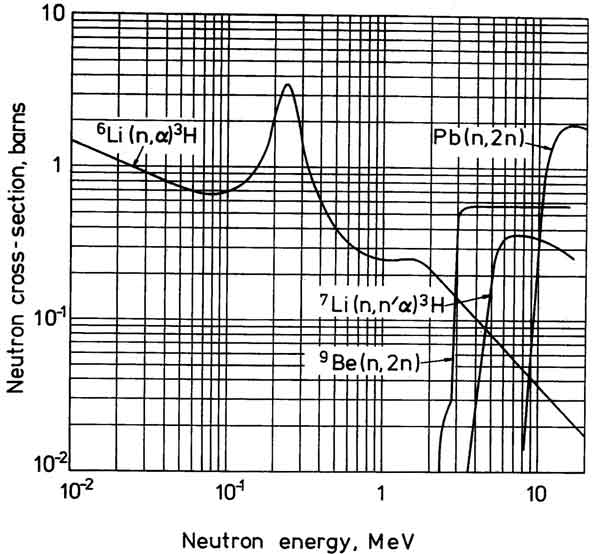
\includegraphics[width=0.8\textwidth]{../images/breeding_xsecs} 
\caption{Cross-sections of various blanket materials. Note the threshold for the \lisev~and neutron multiplying reactions.}
\label{fig:xsects}
\end{figure}

Neutron multipliers such as lead and beryllium not only moderate \SI{14}{\mega\electronvolt} neutrons, yielding a softer neutron spectrum for increased \lisix~reactions, but also generate additional neutrons from (n,2n) reactions. Neutron multiplication materials will be discussed again shortly.

\lisev~interactions with neutrons, being endothermic, possesses a threshold energy below which it will not react with neutrons. It does, however, have a small but significant cross-section (around 1 barn) for neutrons with energies greater than 5 MeV. The \lisev~reaction is:
\begin{align}
\ce{n + ^7Li -> n + He + T}-\SI{2.47}{\mega\electronvolt}\label{eq:Li7T}
\end{align}
where the reaction releases a lower energy neutron which is immediately available for capture by \lisix~atoms. Due to \lisev~ability to act as neutron multiplier, \lio, with a high lithium atom density, is potentially capable of attaining adequate tritium breeding ratios without an external neutron multiplication material. Several atomic densities of lithium for select candidate materials are given in \Cref{fig:li-density}. Aside from \lio~, all ternary oxides require neutron multiplication due to low lithium density.

\begin{figure}[ht]
\centering
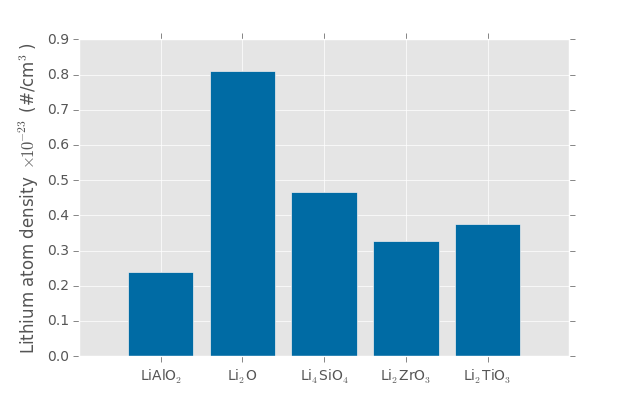
\includegraphics[width=0.8\textwidth]{images/li-density} 
\caption{Lithium oxide is the only ceramic with lithium density sufficiently high to potentially operate without a neutron multiplier. All other ternary oxides have comparable lithium densities.}
\label{fig:li-density}
\end{figure}
 %However, as will be shown next, \lio~has very high tritium solubility to the extent that tritium inventories in \lio~may be unacceptably high.

 %Lithium metal is soft, has a low density (of 0.53 g/cm$^3$), and has a physical appearance similar to lead. 

% Mean-free-path of tritium-producing reaction in natural lithium
% \begin{align*}
% \lambda_t & > \SI{70}{\centi\meter} && n(\SI{14}{\mega\electronvolt})\\
% \lambda_t & \approx \SI{2}{\centi\meter} && n(\SI{1}{\electronvolt}) 
% \end{align*}

% In 90\% enriched \lisix~,
% \begin{align*}
% \lambda_t & \approx \SI{0.15}{\centi\meter} && n(\SI{1}{\electronvolt}) 
% \end{align*}
% \lisix~cross-section at \SI{0.025}{\electronvolt} is %\SI{740}{\barns}.



\subsection{Thermochemical Properties}
Vapor pressure, phase equilibria, thermal stability, and thermodynamics are several of the thermochemical properties important to the study of ceramic breeder materials. 
% Li2O, only ceramic that could possible achieve TBR>1 without dedicated neutron multiplier. Highly hygroscopic.
% Li2O + H2O -> 2LiOH deltaH = 128.9 kJ/mol
% LiOH is highly corrosive

A major concern of candidate materials is the solubility of tritium in the material; too high solubility will lead to unacceptable levels of tritium inventory. A simplified calculation can be performed on the lithium oxides to predict the function of \ce{T2O} partial pressure in gas phase. Assuming: 1) thermochemical data of hydrogen applies to tritium; 2) isotope effects are not considered; 3) tritium exists in the form of \ce{LiOT} in solid solution; and 4) activity coefficients of all species are unity. We can then calculate the partial pressure of oxides as:
\begin{align}\label{eq:liot-equilibrium}
\ce{2LiOT + MO_X <=> Li2MO_{X+1}}
\end{align}
and
\begin{align}
p(T_2O) = X_MX^2K_p
\end{align}
where $p(T_2O)$ is the partial pressure of \ce{T2O}, $X$ is the mole fraction of LiOT, and $X_M$ is the mole fraction of the binary metal oxide (\textit{e.g.} \ce{TiO3}). 

As neutrons transmute lithium from the ceramic, the stoichiometry of the material will begin to change. There is great uncertainty in the activity of lithium-depleted species. The lithium depleted species may not exist in the simple metal oxide form (\textit{e.g.} \ce{Al2O3}) but most probably another ternary compound (\textit{e.g.} \ce{LiAl5O8}). In the examples of lithium aluminate, \ce{LiAl5O8} is more stable than \ce{LiAl2O3} and therefore free energy changes and $k_p$ values for reactions may be overestimated. Moreover, the composition of the breeding material continuously changes during operation of the blanket because of lithium burn-up. Because tritium is being removed from the blanket, the mole fraction of \ce{LiOT} will reach a constant value. However, the concentration of other specie (metal oxides) will continuously increase.

Although there is considerable uncertainty in many of the terms of \Cref{eq:liot-equilibrium}, approximations can be made for many of the candidate ceramics. Equlibrium tritium concentrations in solid ceramic breeders for a \ce{T2O} partial pressure of \SI{1.3}{\pascal} were calculated by Clemmer and his results are reproduced in \Cref{fig:solubility}.\cite{Clemmer1980} From estimates of solubility shown in \Cref{fig:solubility}, it is immediately apparent that all the ternary oxides have significantly lower tritium ``solubilities'' than \lio. In spite of the promising feature of \lio~being capable of existing without a neutron multiplier due to its high lithium density, the tritium inventory of the material may be unacceptably high.

\begin{figure}[ht]
	\centering
	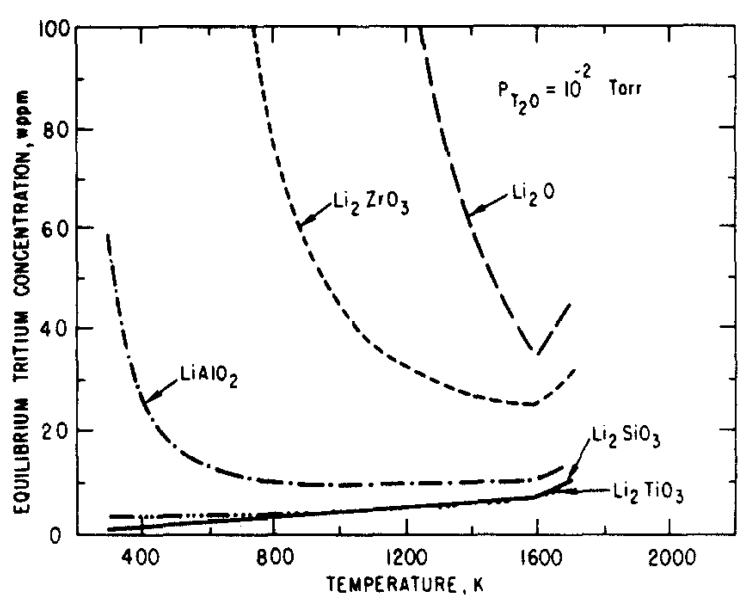
\includegraphics[width=0.75\textwidth]{images/solubility} 
	\caption{Calculated equilibrium tritium concentrations in candidate solid breeding materials at $P_{T_2O} = \SI{1.3}{\pascal}$.}
	\label{fig:solubility}
\end{figure}



% Lastly, because safety as a key issue supporting fusion reactors, we must consider that lithium is chemically reactive with oxygen. Two interactions are:
% \begin{align*}
% 2\mathrm{Li} + \frac{1}{2}\mathrm{O} &\rightarrow \mathrm{Li}_2\mathrm{O} - 142.75~\text{kCal/mol}\\
% 2\mathrm{Li} + \mathrm{O} &\rightarrow \mathrm{Li}_2\mathrm{O}_2 - 151.9~\text{kCal/mol}
% \end{align*}
% Lithium will exothermically react with water (or air, concrete, or any moisture-containing materials) with high amounts of energy released. Of primary concern in lithium fires is the peak flame temperature. This will determine, to a large extent, whether many radioactive species become air-borne by vaporization. The flame temperature depends on many variables. Some investigations found it to be about \SI{2500}{\kelvin} which would cause some materials to melt but not vaporize.

%Vaporization data for several candidate ceramics is discussed by Johnson \textit{et al.}.\cite{Clemmer1980}; showing that higher lithium vapor pressures exist for materials with higher lithium content.

\subsection{Tritium Release and Recovery}
Tritium recovery from solid tritium-breeding materials is a key factor in establishing the viability of the solid-breeder concept. Designs of solid breeders have tritium removed with a purge gas (primarily helium) flowing through the open porosity of packed beds of lithium ceramics. The feasibility of the solid breeder concept is based on the capability of tritium to readily transport from the solid ceramic into the purge gas. Tritium release is a function of grain size, microsctructure, and open/closed porosity. To understand the capability of tritium removal, five mechanistic steps are identified for bred tritium to be recovered (visualized in \Cref{fig:mechanisms_tritium_transport}) . The steps follow as
\begin{enumerate}
\item bulk diffusion,
\item desorption of tritium (T$_2$O),
\item grain boundary migration,
\item percolation of tritium through pores internal to the solid ceramic toward the flowing purge gas,
\item convective mass transfer out of the blanket via purge channels.
\end{enumerate}

\begin{figure}[ht]
	\centering
	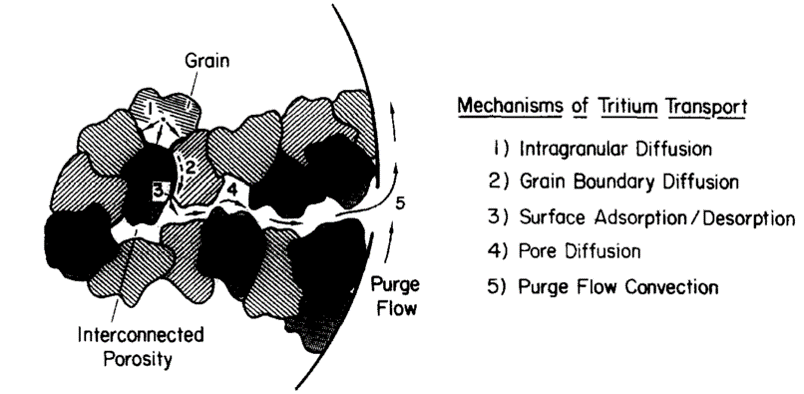
\includegraphics[width=0.75\textwidth]{images/mechanisms_tritium_transport} 
	\caption{Mechanistic steps of tritium transport through ceramic materials into the purge gas for removal.}
	\label{fig:mechanisms_tritium_transport}
\end{figure}

Bulk diffusion of tritium is considered to be a significant contributor to tritium inventory. For spherical particles of radius $r_p$, assuming zero surface concentration, the tritium inventory $T$ is given by 
\begin{equation}\label{eq:inventory-diff}
T = \frac{1}{15}\dot{T}\frac{r_p^2}{D}
\end{equation}
where $\dot{T}$ is the tritium generation rate and $D$ is diffusivity of tritium in the ceramic. It is significant to note that the tritium inventory is a function of the square of the particle size. Thus it is clear that: (i) small grain sizes are required for minimum tritium inventory and (ii) grains should not significantly grow during the lifetime of a reactor blanket. Diffusivity values of tritium in ceramics are extremely scarce and with much uncertainty. Kinetic experiments of post-irradiation tritium release from several candidate breeders have been performed. The kinetics in the experiments are non-steady-state and the diffusivity is given by 
\begin{equation}\label{eq:exp-diff}
D = 0.16 \frac{r_p^2}{\tau}
\end{equation}
where $\tau$ is the mean residence time, defined as the time required to extract 87.4\% of the tritium. Combining \Cref{eq:inventory-diff} and \Cref{eq:exp-diff} eliminates diffusivity and radius (with large variation between particles and grains), yielding:
\begin{equation}
T = 0.42 \dot{T}\tau
\end{equation}

We can then estimate the diffusive inventory in a blanket based on the readily-measured residence time, $\tau$. It must be kept in mind that the particular micro-structure of the ceramics measured in kinetic experiments must correspond to the micro-structure of the material in the blanket in order for the diffusivity predictions to hold. In other words, residence times of \SI{1}{\milli\meter} \lit~with average grain sizes of $\mu = \SI{1}{\micro\meter}$ are utterly inappropriate to calculate tritium diffusion in \SI{0.5}{\milli\meter} pebbles of \lis~with average grain sizes of $\mu = \SI{5}{\micro\meter}$, for example.

The tritium generation rate, $\dot{T}$ is a function of the fusion reactor power output and blanket design. Assuming this value is known for a given blanket, residence times have been measured to be temperature dependent which is consistent with diffusion-controlled processes. Therefore, based on the present model, the range of operating limitations are defined on the low end where bulk diffusion is the rate-limiting step. A minimum temperature is defined as the temperature at which the tritium inventory exceeds \SI{1}{\kilo\gram\per\giga\watt}. The minimum temperatures for many candidate materials are shown (with slight variation between sources) in \Cref{fig:Tmin}. Minimum temperatures generally range from 300 up to \SI{400}{\celsius}.

\begin{figure}[ht]
	\centering
	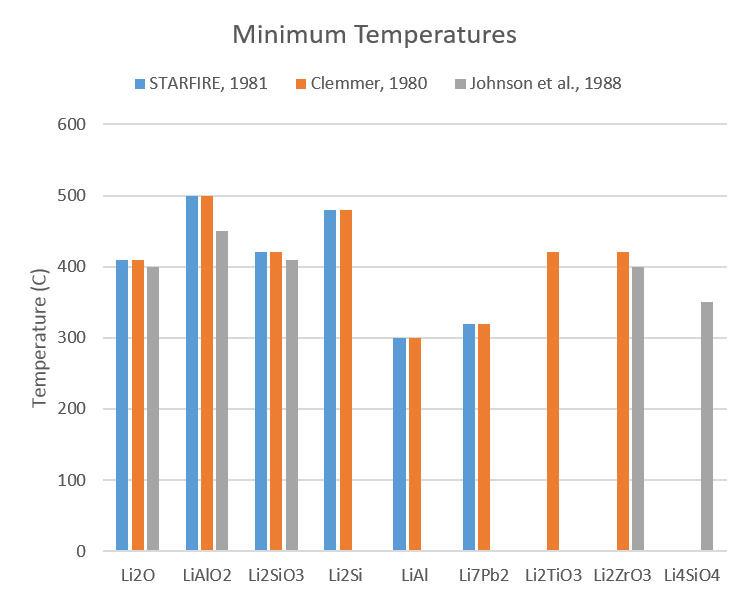
\includegraphics[width=\textwidth]{images/Tmin} 
	\caption{Minimum temperatures for various candidate materials (compiled from various sources) based on rate-limiting diffusion processes.}
	\label{fig:Tmin}
\end{figure}

As we saw from \Cref{eq:inventory-diff}, tritium inventory goes with the square of grain size and thus another operating limit on temperature arises. An upper limit of temperature is based on restructuring or grain growth in ceramics which can greatly affect the diffusive inventories. When ceramic materials are heated above their sintering temperature, generally in excess of $0.8 T_\text{melt}$ (in absolute temperature), grains will grow. The effects of sintering at \SI{1200}{\celsius} over a number of hours is shown in \Cref{fig:material-production-NFRI} (images courtesy of Yi-Hyun Park from NFRI). Grain growth, as witnessed in these images, must be avoided in operation.

\begin{figure}[ht]
	\centering
	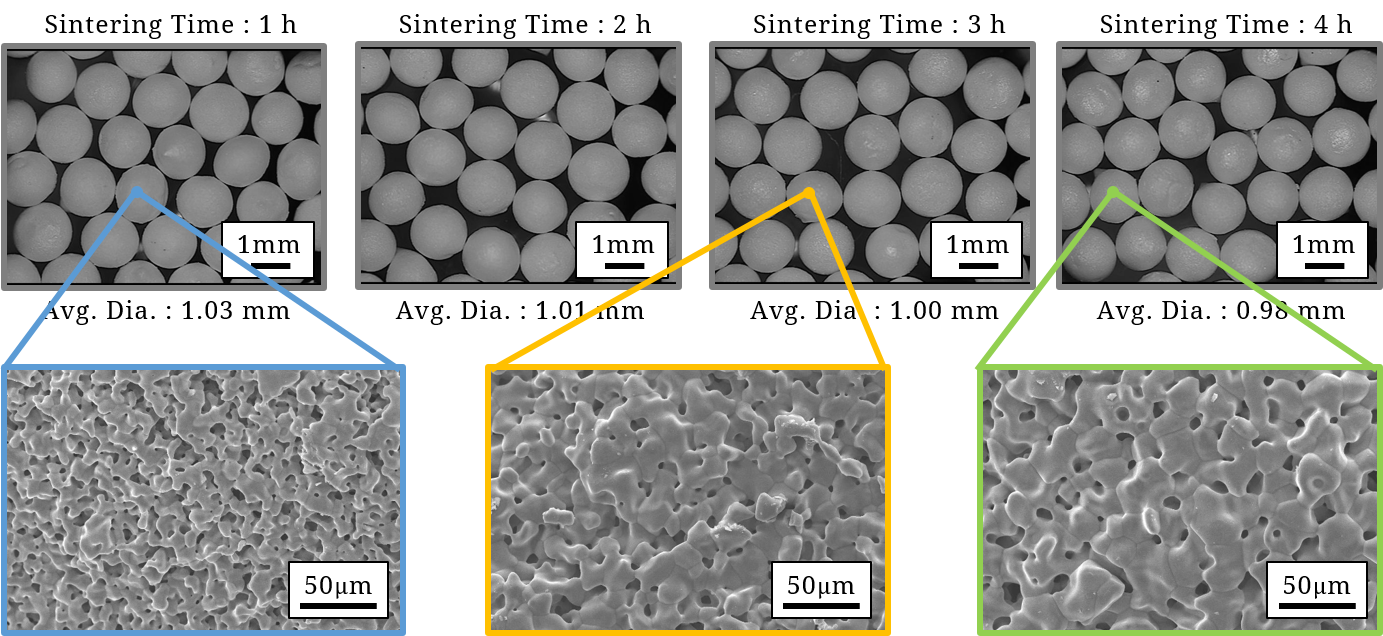
\includegraphics[width=\textwidth]{images/material-production-NFRI} 
	\caption{Maximum temperatures for various candidate materials (compiled from various sources) based on irradiated sintering temperatures ($0.6T_\text{melt}$).}
	\label{fig:material-production-NFRI}
\end{figure}

Moreover, neutron radiation typically enhances sintering characteristics and lowers sintering temperatures; effects of radiation are expected to reduce the sintering temperature to $0.6 T_\text{melt}$.\cite{Johnson1981} Maximum temperatures are thus set by sintering considerations. Candidate materials are compared in \Cref{fig:Tmax}. In general, keep in mind that acceptable candidate materials have their maximum temperature between 750 and \SI{900}{\celsius}. 

\begin{figure}[ht]
	\centering
	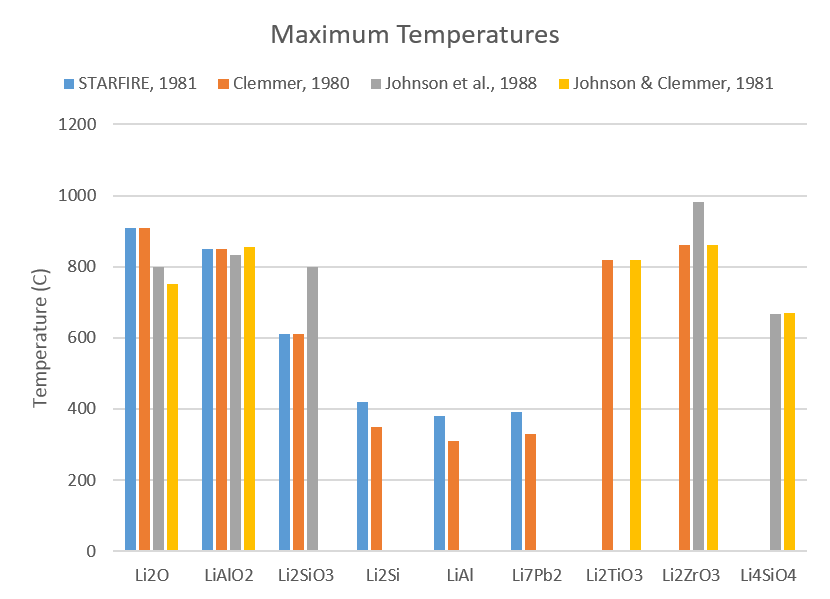
\includegraphics[width=\textwidth]{images/Tmax} 
	\caption{Maximum temperatures for various candidate materials (compiled from various sources) based on irradiated sintering temperatures ($0.6T_\text{melt}$).}
	\label{fig:Tmax}
\end{figure}

As a consequence of the tritium inventory of solid breeder material, we are faced with a relatively narrow operational temperature to which solid breeder designers must adhere, roughly between 350 and \SI{800}{\celsius}. Thus to provide designers the ability to optimize breeder volumes for tritium breeding and subsequent tritium release, we must understand the important physics and phenomena dictating thermophysical properties and thermomechanical responses of pebble beds during operation in a fusion reactor. Thermomechanical modeling of solid breeder pebble beds remains an important field in solid breeder research and much of Chapter 2 will focus on this topic.


\FloatBarrier
\subsection{Physical \& Thermophysical Properties}
The temperature window established for tritium release dictates the thermal characteristics of pebble beds become critically important to understand. Candidate ceramic materials is itself quite low, being reduced by porosity. Several candidate conductivities are given in \Cref{fig:k_s} assuming 80\% theoretical density; \lit~has comparable conductivities with \lis.

\begin{figure}[ht]
	\centering
	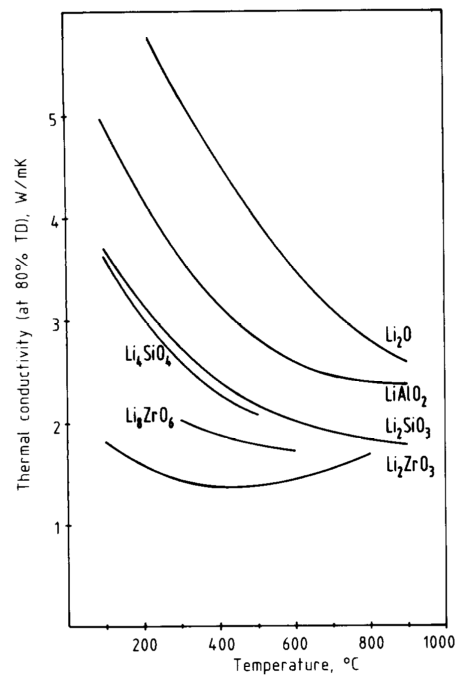
\includegraphics[width=0.45\textwidth]{images/k_s} 
	\caption{.}
	\label{fig:k_s}
\end{figure}

The Young's modulus for ceramic materials 
% The material integrity is a function of pebble size distribution, sphericity, mechanical strength, chemical stability.
% \lit~has acceptable Li density, not hygroscopic, has lower activation, similar T release to \liz. Mechanically stronger than \lis.
% \lis~has weak crush strength, acceptable Li density, stable (can't read my notes)

\FloatBarrier 
\subsection{Compatibility}
Compatibility studies have been carried out at several temperatures between various pairs of breeder and structural materials.\cite{Johnson1988} \ce{Li5FeO4}, \ce{Li2CrO2}, and \ce{Li2Ni8O10} were common corrosion products (varying by structural material). \lio~was seen to be most reactive; reaction rates for \lis, \liz, and \lial~were much lower. However, in studies of \lio~where the material was rigorously freed of moisture impurity, \lio~was found to be inert to metals. Corrosion properties of \lio~are therefore attributed to the presence of highly corrosive LiOH contamination happening in the presence of water with \lio. In general, reaction rates increase with increasing temperature and moisture content.\cite{Johnson1991} From structure-ceramic compatibility point of view, ternary oxides such as \lit~and \lis~are more desirable.

Compatibility of ceramic materials with neutron multiplying materials is also necessary to understand. Interaction of ternary oxide ceramics with beryllium was found to be counter to expectations based on thermodynamics and seen to be negligible up to \SI{650}{\celsius} for \lis, up to \SI{700}{\celsius} for \lial~and \liz, for durations up to 3000 hours. A beryllium oxide layer is assumed to form on the material surface, thereby protecting it from further oxidation. The SIBELIUS experiment studied the effect of neutron irradiation on the \ce{BeO} layer. Data from SIBELIUS indicate the beryllium oxide layer appears to have some influence on the amount of tritium retained by the beryllium discs. The tritium release from the ceramics, on the other hand, is consistent with other tritium release measurements of the ceramic materials in the absence of beryllium and therefore appears to not be affected by adjacent beryllium.\cite{Kopasz1995,Roux1992} 

Recently, advanced neutron multiplier material has been considered which overcomes some compatibility issues with pure beryllium. For example, beryllides (such as \ce{Be12Ti}) offer higher melting point, better compatibility than pure beryllium, significantly lower tritium inventory, and sufficiently high tritium breeding ratios.\cite{Kawamura2003a} Development of advanced materials continues to be a rich bed of research.

\subsection{Radiation Effects}
We have already discussed the anticipated effect of radiation on lowering predicted sintering temperatures of candidate ceramic materials. While in a fusion reactor, the ceramic materials will subjected to high temperatures and changing material characteristics from the neutron environment. The neutron capture reaction of \ce{n + ^6Li -> T + He} produces significant lattice damage during irradiation.\cite{Johnson1981} Not only are two large gas atoms produced, one of which is not expected to be soluble in the parent material, but also a lithium vacancy is produced. Several anticipated radiation damage mechanisms are:
\begin{itemize}
\item Displacement Damage
	\begin{itemize}
	\item Vacancies
	\item Loops, Clusters, etc.
	\item Interstitials
	\end{itemize}
\item Reaction Products
	\begin{itemize}
	\item Bubbles
	\item Interstitials
	\item Substitutional Defects
	\end{itemize}
\item Lithium Depletion
	\begin{itemize}
	\item Vacancies
	\item Oxygen Excess
	\item Nonstoichiometry
	\end{itemize}
\item Microstructural
	\begin{itemize}
	\item Sintering
	\item Grain Growth
	\item Microcracking
	\end{itemize}
\end{itemize}
and the manifestation of these atomistic changes as microstructural damage must be evaluated with irradiation experiments.

In lithium ceramics there are a minimum of two sublattices composed of anions and cations. Creation of more defects on one sublattice than the other, for instance on the oxygen lattice, would lead to charge separation within the matrix. If sufficient defect mobility exists, the newly formed defects can annihilate or cluster, forming voids or precipitates within the crystal. Displacement damage to lattices is quantified with a value displacements per atom, dpa. In fusion reactors, solid breeder materials will receive substantial displacement damage from high energy neutrons of the plasma. Fusion neutrons that have been slowed (from interaction with neutron multiplication or structural materials) to lower energies will produce much less displacement damage.

Helium generated in the solid breeder material during irradiation, owing to its inert nature, will have a much lower solubility in ceramics than tritium, since only interstitial positions are available. The lower solubility for helium will result in a lower permeability so that the rate of migration out of the lattice will be less. Moreover, low solubility will enhance bubble formation and swelling. Swelling can have significant negative consequences on the mechanical stability of ceramic pebbles.

A consequence of neutron capture is loss of lithium atoms from ceramic lattices. This loss creates either a lithium vacancy or a localized excess of oxygen, \textit{i.e.} oxygen interstitials. Since tritium ions are created during the neutron capture of a lithium ion, the overall electrostatic equilibrium of the crystal is maintained. When the tritium ions are subsequently released to the purge gas, it necessarily follows that the oxygen ions must also be released in order to avoid a charge buildup in a single valency system. If multivalent ions (\textit{e.g.} \ce{Fe^{+2}}, \ce{Fe^{+3}}) are present, then a change in oxidation states would balance the charge of the excess oxygen. From this point of view, it is natural that we observe tritium released as \ce{T2O} in \lio~systems rather than as a hydrocarbon or \ce{T2}.\cite{Johnson1981}

Lastly, as discussed in the discussion of thermochemistry of candidate ceramics, as lithium depletion (or lithium burn-up) occurs to a significant extent (around 5\%), the resultant nontsoichiometry in ternary oxides could establish rather than single-phase condition. For example, under irradiation and lithium burn-up, \lis~would lead to an excess of silica and the melting point of the \SI{1300}{\celsius} to a eutectic temperature of \SI{1024}{\celsius}. Such a reduction in melt temperature would have significant impact on sintering and tritium inventory in the solid breeders.\cite{Johnson1981}

This list of irradiation effects is by no means complete and irradiation experiments are ongoing.\cite{vanderLaan200099} Moreover, experiments that can recreate fusion neutron sources are necessary steps towards realizing solid breeder technology.\cite{Abdou1996d}

\section{Neutron Multiplication in Solid Breeders}
Because neutron multiplying material is a necessity for all ternary oxides, we will discuss some of the important aspects of neutron multiplication materials. Beryllium is identified as the most suitable material for neutron multiplication in solid breeders. The common reaction of \ce{9Be} is:
\begin{align}
\ce{n + ^9_4Be -> 2n + 2He + T}-\SI{1.57}{\mega\electronvolt}\label{eq:Be-n}
\end{align}

The following reaction also has small probability of occurrence (check cross-section for this reaction)
\begin{align*}
\ce{n + ^9_4Be -> ^4He + ^6He} \\
\ce{^6He -> ^6Li + beta^-} \\
\ce{n + ^6Li -> He + T}
\end{align*}

The melting temperature of natural beryllium is \SI{1250}{\celsius}, advantageous for solid form of neutron multiplier with solid tritium breeder. Aside from pure beryllium, other options have been considered. Beryllium will also exist as a pebble bed. 

A short list of salient points:
\begin{itemize}
\item{\ce{Be} incompatibility with structure steel, forming \ce{FeBe13}}
\item{\ce{Be} reaction with water forming \ce{BeO} (\ce{Be + H2O -> BeO + H2})}
\item{\ce{Be} reaction with oxygen forming \ce{BeO} (\ce{2Be + O2 -> 2BeO})}
\begin{itemize}
\item{\ce{BeO} has excellent compatibility with structural steel}
\item{\ce{BeO} is a carcinogen, causes beryllium disease if inhaled}
\end{itemize}
\item{Diffusional release of T from irradiated beryllium is very slow}
\end{itemize}

As discussed previously, an alternative to pure beryllium that has been receiving much attention lately is the beryllide of \ce{Be12Ti}. The advantages of this material include:\cite{Kawamura2003a}
\begin{itemize}
\item{more compatible with steel than \ce{Be}}
\item{less swelling than \ce{Be}}
\item{tritium inventory of beryllide is significantly lower than \ce{Be}}
\item{high \ce{Be} density maintains neutron multiplication characteristics (sufficiently high tritium breeding ratio)}
\end{itemize}

Lastly, we must bear in mind limited abundance of \ce{Be} on Earth (remember Homework set). Thus we must be economical in our consumption of beryllium for neutron multiplication in fusion reactors.

\subsection{Fabrication}
One last point to discuss on ceramic materials before moving on to a discussion of neutron multipliers concerns fabrication. Candidate ceramic material feasibility is in part dependent on the fabrication price and ability to scale to industrial output quantities. While this is an important point for realization of solid breeders, it will not be discussed in detail here. van der Laan \textit{et al.}\cite{vanderLaan200099} and Johnson \textit{et al.}\cite{Johnson1991} provide thorough descriptions and discussions for various fabrication techniques.



































\chapter{Introduction to Solid Breeder Designs}
The solid breeder concept with sphere-pac beds satisfies the requirements of a breeder unit: transmute lithium into tritium, act as shield to other sensitive equipment and personnel, and convert energy into extractable heat for electricity production. Common features of pebble bed designs are:
\begin{enumerate}
\item{Always separately cooled with (with \textit{e.g.} helium or water)}
\item{Necessity of neutron multiplication}
\item{Surrounded by a structure of reduced-activation ferritic steel}
\end{enumerate}
In a typical solid breeder module, the module is subdivided into several alternating layers of neutron multiplication material (generally beryllium) and tritium breeding material. The layers are separated by steel plates with internal channels for coolant. A conceptual design of the Japanese solid breeder for ITER is shown in \Cref{fig:japanese-breeder-design}.

Pebble bed forms of tritium breeding volumes have several advantages which include: large surface area to volume, ease of assembly of granular materials into complex geometries, bred tritium can be readily removed with large open porosity between pebbles, and temperature gradients across any single pebble are small enough to avoid damage from thermal stress.

\begin{figure}[ht]
	\centering
	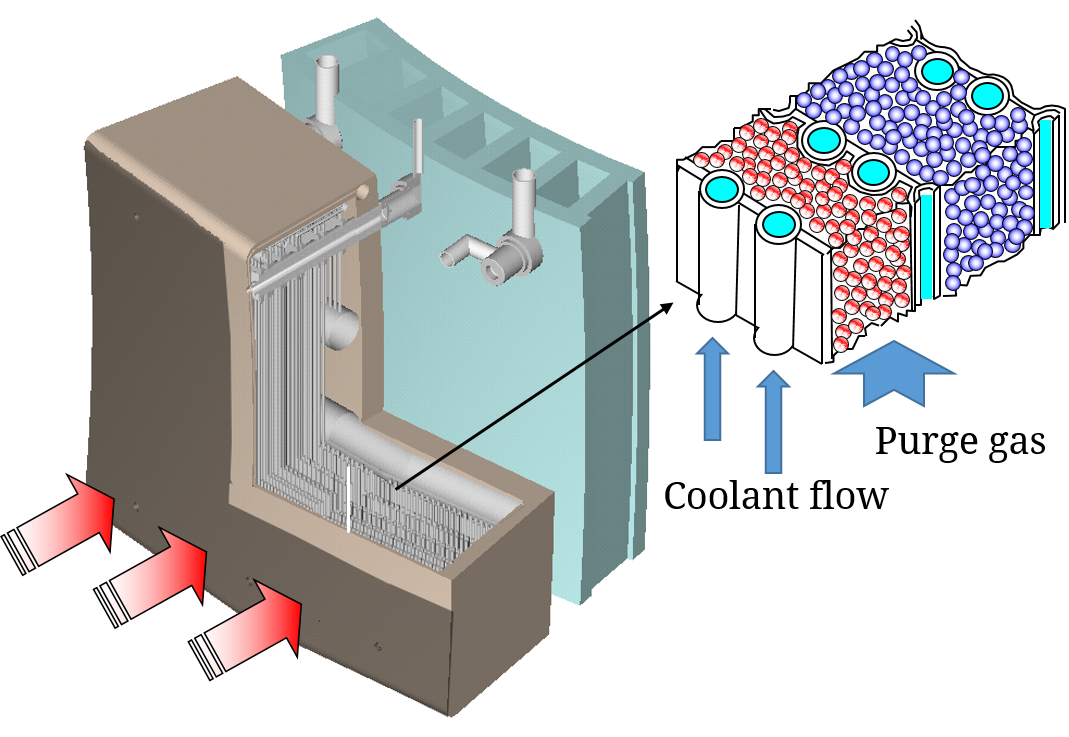
\includegraphics[width=0.6\textwidth]{images/japanese-breeder-design} 
	\caption{Sketch of a typical unit of a pebble bed tritium breeding zone. The pebble bed is cooled with contact to the containing structure.}
	\label{fig:japanese-breeder-design}
\end{figure}

In this chapter, we will review the need for accurate thermal management in solid breeders. We will then present engineering analysis considerations for the interstitial purge gas and fluid coolant as they are necessary for solid breeder design. Following that we will introduce phenomenological models of effective material properties for packed beds, experiments from which constitutive equations can be derived, and solid breeder modeling tools.

\section{Solid Breeder Thermal Management and Imposed Temperature Window}

Tritium breeding blankets will experience high volumetric heating as deposited by high-energy neutrons that are carrying away approximately 80\% of the fusion reaction energy in addition to heating from secondary $\gamma$ rays. Heat deposited in breeders must be transported through pebble bed regions into the walls of containing structures, then ultimately into the coolant gas. Heat deposited into pebble beds will transfer \textit{via} inter-particle contact conduction, inter-particle radiation, and convection with the helium purge gas. At the interface with the structural material, similar modes of heat transfer are present: particle-wall contact conduction, particle-wall radiation, and communication \textit{via} helium purge gas convection. There exists a coupling between mechanical forces acting upon beds and their heat transport capabilities and we must consequently understand packing structures in order to understand heat transfer.

The structure of packed beds can be considered as a metastable configuration that will last indefinitely unless acted upon by an external perturbation such as vibration or compressive pressure.\cite{Jaeger1996} The ability of a metastable configuration to resist perturbations can, in some way, be quantified by the initial packing fraction. For more compliant beds (lower packing fractions), stresses from thermal expansion can cause significant rearrangement of the packing structure which is not recoverable after stress removal. This phenomena has been observed in numerous experiments as so-called plastic rearrangement of pebble beds.\cite{Reimann:2002kl,Reimann:2000tw,Zhang2015} Plasticity of beds may have significant consequences for the ability of the pebble bed to maintain contact with the containing structure and routes for heat out of the bed due to gap formation between pebble volumes and coolant walls. As the pebbles heat under the nuclear load, thermal expansion of the pebbles in the packed volume will be contained by cooler structural material. Confined expansion will give rise to increased contact pressure between pebbles. Moreover, increased pressure between pebbles can cause, among other effects, brittle pebbles to fragment.

Some amount of restructuring of pebble beds (and internal contact force networks) are also likely to occur from crushing/cracking of individual pebbles, or the effects of inter-pebble sintering and creep arising from the high-temperature, high-stress environment in a breeder unit. Contact conduction in beds, intimately linked to the packing structure, will be impacted during operation of ceramic pebble beds in fusion reactors. Concurrently, interaction of the slow-moving purge gas with tightly packed pebble beds is an additional route of heat transfer that must be understood. Thus, heat transfer in pebble beds is quite different from standard solid materials and requires specialized modeling of the synergistic physics. Knowledge and characterization of thermal transport must anticipate changes to the heat transfer capabilities and predict temperature profiles for pebble bed packing structures that will emerge after initially-packed pebble beds react to prolonged exposure to fusion reactor environments.

We saw earlier that tritium inventory requirements impose a relatively narrow operational temperature window on lithium ceramic pebble beds. Given the high power densities in fusion power reactors, it is therefore necessary to have accurate knowledge of ceramic pebble bed thermomechanical behavior and comprehensive characterization; reliable models of heat transfer in solid breeders are critical for solid breeder designs. In addition, due to the complicated nature of granular materials, heat transfer in these solid breeder volumes remains transient during fusion operation. 

\section{Purge Gas and Coolant Flow}
All heat deposited into the ceramic pebble beds is conducted towards the structure and into coolant. Coolant proceeds out of the tritium breeding module and into a standard electricity production cycle where heat is extracted. After tritium is generated inside the ceramic, the bred tritium is ultimately carried away by a low-pressure, slow moving purge gas (primarily helium) and extracted in a closed loop for fuel. A sketch of a generic volume of ceramic pebble bed is given in \Cref{fig:solid-breeder-sketch}

\begin{figure}[ht]
	\centering
	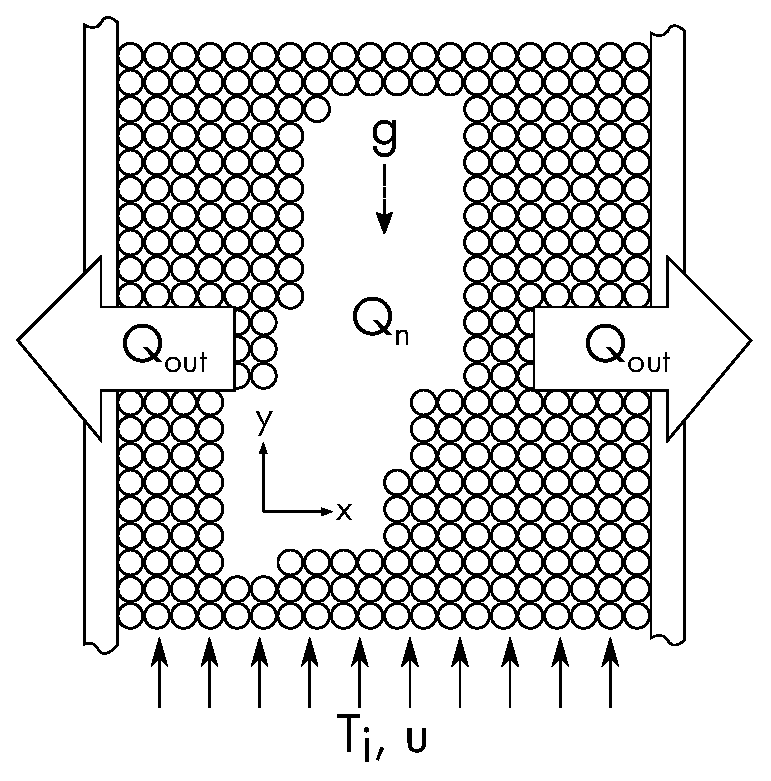
\includegraphics[width=0.6\textwidth]{images/x-domain} 
	\caption{Sketch of a typical unit of a pebble bed tritium breeding zone. The pebble bed is cooled with contact to the containing structure.}
	\label{fig:solid-breeder-sketch}
\end{figure}


\subsection{Purge gas}
The purge gas composition is generally helium with small amounts of hydrogen which promotes tritium release from ceramics. Flow rates of purge gas are kept low to minimize the pressure drop across tightly packed pebble beds.

Pressure drop (per unit length) for the purge gas can be calculated based on the Kozeny-Carman correlation; derived for packed beds at the close-packed limit,
\begin{equation}\label{eq:K-C-pressure}
    \frac{\Delta p}{L} = \frac{180 \bar{U} \mu}{d_p^2} \frac{(1-\epsilon)^2}{\epsilon^3}
\end{equation}
where $\mu$ is the viscosity, $\epsilon$ is the void fraction, $d_p$ is the particle diameter (assuming spherical) and $\bar{U}$ is the superficial velocity of the fluid in the packed bed.

Carman points out the limitations of applicability of the Kozeny-Carman (KC) equation: built into the equation is the assumption that the range of pore size and shape is fairly isotropic and similarly the tortuosity through the packed bed is relatively uniform. Pressure drop as a function of Reynolds number for \SI{1}{\milli\meter} particles in a packing fraction of $\phi = 1-\epsilon = 0.645$ in helium at \SI{600}{\celsius} is given in \Cref{fig:KC-pressure-drop}.

\begin{figure}[ht]
    \centering
    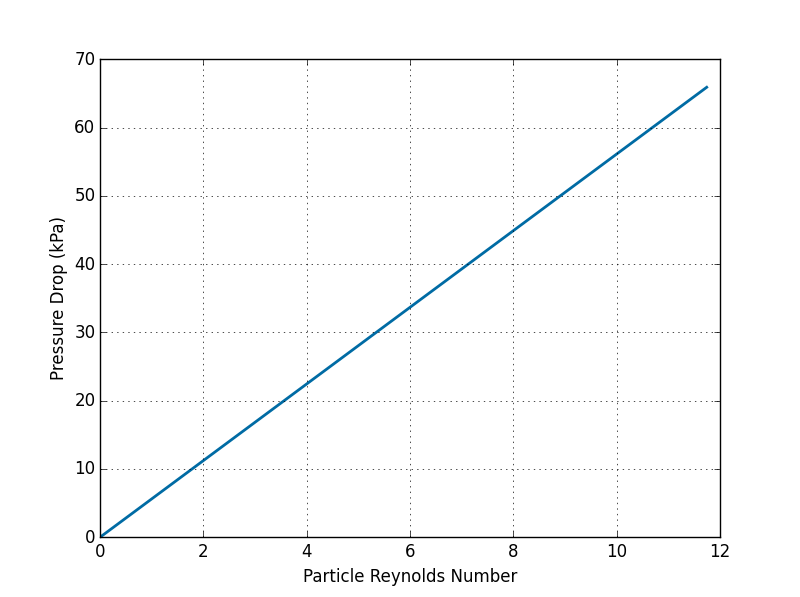
\includegraphics[width=0.75\textwidth]{images/KC-pressure-drop}
    \caption{Kozen-Carman pressure drop increases linearly with particle Reynolds number.}
    \label{fig:KC-pressure-drop}
\end{figure}

Tritium permeation from the purge gas through piping is a safety concern for solid breeders. Tritium extraction and permeation will be covered in another lecture of this class.

\subsection{Coolant}
The function of coolant is not only to maintain ceramic breeder volumes within specified temperature windows and keep structural materials under their operable limits, but also to extract high-quality heat for power generation. Current tritium breeding designs call for a high pressure helium, approximately 8 MPa. Inlet temperatures of coolant are sufficiently high to maintain the minimum temperature of breeder volumes, coolant inlets are approximately \SI{300}{\celsius}. The coolant is run such that the outlet is held around \SI{500}{\celsius}; obeying concerns for structural integrity of the steel container that happen around \SI{600}{\celsius}.

Analysis of the coolant is nothing exotic. We can apply standard engineering practices of heat transfer in a fluid duct such as the Dittus-Boelter equation for obtaining Nusselt number,
\begin{equation}
\text{Nu}_D = 0.023 \text{Re}_D^{4/5}\text{Pr}^{0.3}
\end{equation}
where the equation is valid for Re$\ge 10000$ and the Nusselt and Reynolds numbers are based on the hydraulic diameter of the duct.

Lastly, one special consideration for the coolant are the safety issues of high pressure coolant stressing the structure or chemically reacting (or transporting tritium) during a breach. These concerns are specific to each tritium breeding volume and are often modeled before licensing is allowed for designs.


\section{Phenomenological Properties of Packed Beds}
One approach to studying heat transfer granular material is to treat the packed bed as a fictitious continuous media. Many experiments have been carried out for developing phenomenological models of effective material properties. In this approach, heat transport in pebble beds is often characterized with an effective thermal conductivity, $k_\text{eff}$, and interface heat conductance. Many models have shown their ability to accurately predict the temperature profiles for pebble beds under specific operating conditions. We begin with a review of $k_\text{eff}$ correlations.

\subsection{Empirical Models for Packed Beds}
Deissler and Boegli, in 1958, proposed upper and lower bounds of effective thermal conductivity, $k_\text{eff}$, in two-phase granular media to be given by alternating layers of the two phases arranged in parallel or series, respectively \cite{Deissler1958}. In the case of parallel layers, effective conductivity, normalized by fluid conductivity, is
\begin{equation}\label{eq:keff-parallel}
	\frac{k_e}{k_f} = \epsilon + (1-\epsilon)\kappa
\end{equation}
where $k_f$ is the fluid conductivity, $\kappa = k_s/k_f$ is the ratio of solid to fluid conductivity, and $\epsilon$ is the void fraction in the porous media. Similarly, the minimum effective conductivity is found in a serial layering of the solid and fluid phases,
\begin{equation}\label{eq:keff-series}
	\frac{k_e}{k_f} = \frac{1}{\epsilon + (1-\epsilon)/\kappa}
\end{equation}
\Cref{eq:keff-parallel,eq:keff-series} act as theoretical upper and lower limits to true effective thermal conductivities of real material.

One of the most widely-used correlations was put forth by Zehner and Schlunder in 1970 \cite{Zehner1970,Zehner1972}. They considered a cylindrically-shaped unit cell and made the analogy between heat and mass transfer to derive an empirical fit to data in the bulk of two-phase porous media. The Zehner-Schlunder (ZS) correlation is
\begin{equation}
    \frac{k_e}{k_f} = \left(1-\sqrt{1-\epsilon}\right)+\frac{2\sqrt{1-\epsilon}}{1-B/\kappa}\left[\frac{(1-1/\kappa)B}{(1-B/\kappa)^2}\ln\left( \frac{\kappa}{B} \right) - \frac{B+1}{2} - \frac{B-1}{1-B/\kappa}\right]
\end{equation}
where $B$ is a deformation parameter related to porosity as
\begin{equation}\label{eq:zs-B}
    B = 1.25\left(\frac{1-\epsilon}{\epsilon}\right)^{1.11}
\end{equation}

Over the years, many other correlations have been developed for predicting effective conductivity of packed beds. Some focus on conditions of higher porosity, consider radiation effects, or situations of large $\kappa$. A number of correlations have been plotted together along with the three presented here; given in \Cref{fig:kappa-experimental-comet}. Plotted on the figure is also a compilation of experimental data from many sources (reproduced from Ref.\cite{VanAntwerpen2010}) and recent COMET data recorded for graphite material at UCLA.

\begin{figure}[ht]
    \centering
    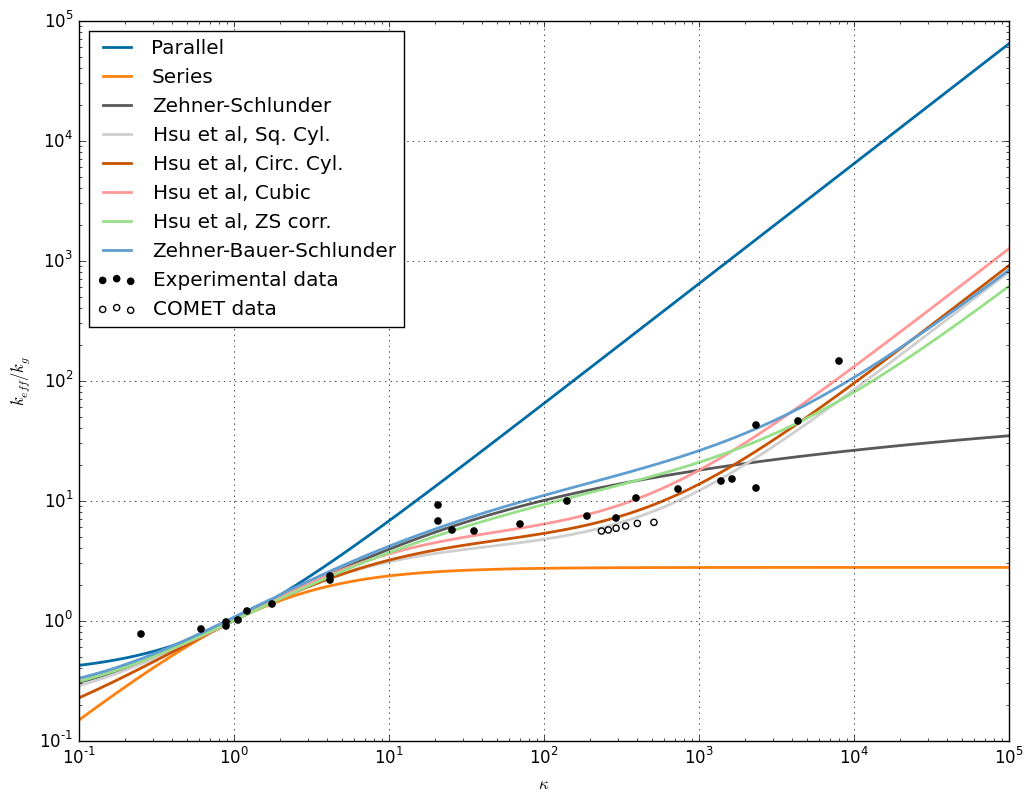
\includegraphics[width=\textwidth]{images/keff-kappa-experimental-comet}
    \caption{Comparison of COMET data on IG11 graphite, $k_\text{eff}$ correlations, and experimental data. Data compiled by \cite{VanAntwerpen2010} from many sources and measured data at UCLA.}
    \label{fig:kappa-experimental-comet}
\end{figure}

\subsection{Experimental Measurements of Lithium Ceramics}
Effective conductivities have been measured for several candidate ceramics. A reliable technique for measuring conductivity in packed beds is with a hot-wire technique; the technique is thoroughly described in ASTM standard C1113/C1113M document. Briefly, hot-wire measurements are done by raising the temperature of a pebble bed up to a background value (the reported value of $k_\text{eff}(T)$), then pulsing an electric current through a wire embedded in the bed. The pulse of heat on the wire decays as energy is conducted into the pebble bed. The rate of decay provides information on effective thermal diffusivity and thermal conductivity of the packed bed. A sketch of a hot-wire setup and the current setup at UCLA is shown in \Cref{fig:HWT}.

\begin{figure}[h]
	\centering
	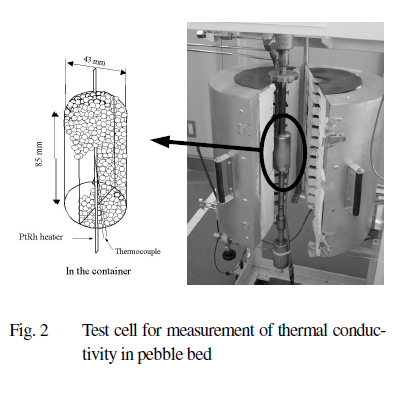
\includegraphics[trim={0cm 2cm 0cm 0cm},clip, width=0.75\textwidth]{images/HWT} 
	\caption{Schematic of hot wire embedded in a pebble bed and the realization in UCLA's lab (right).}
	\label{fig:HWT}
\end{figure}

Many experiments have been run to measure the effective thermal conductivity of a volume of ceramic pebbles. In \Cref{fig:keff}, the effective conductivity is seen to be strongly affected by the interstitial gas but weakly affected by the mechanical loads on the bed. The main conclusions to bear in mind from \Cref{fig:keff} are that: 1) the interstitial gas is an important transporter of heat in the bed and 2) the effective thermal conductivity of the pebble bed is low and will limit the size of the ceramic pebble bed volume to satisfy the temperature window imposed on ceramic breeders.

\begin{figure}[h]
        \centering
        \begin{subfigure}[t]{0.45\textwidth}
                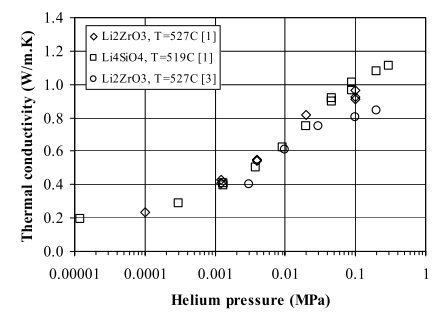
\includegraphics[width=\textwidth]{images/keff-pressure}
                \caption{Effective conductivity of ceramic pebble beds is dependent on the pressure of the interstitial gas below the Knudsen limit.}
                \label{fig:keff-pressure}
        \end{subfigure}%
        ~
          %add desired spacing between images, e. g. ~, \quad, \qquad, \hfill etc.
          %(or a blank line to force the subfigure onto a new line)
        \begin{subfigure}[t]{0.45\textwidth}
                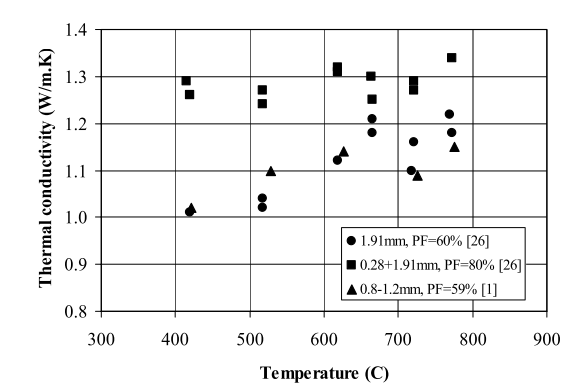
\includegraphics[width=\textwidth]{images/lit-keff-exp}
                \caption{The effective conductivity of pebble beds is weakly dependent on external mechanical pressure.}
                \label{fig:keff-lit}
        \end{subfigure}
        \caption{Effective conductivity of lithium ceramics. Results from Ref.~\cite{Abou-Sena2005}}\label{fig:keff}
\end{figure}

Measurements for \lis~and \lit~are given in \Cref{fig:k_eff} for different interstitial gases and packed bed temperatures. In a stagnant helium environment, the effective conductivity values for both materials fall to around \SI{1}{\watt\per\meter\per\kelvin}.

\begin{figure}[h]
	\centering
	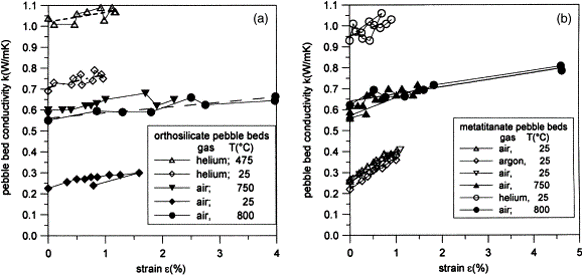
\includegraphics[width=0.85\textwidth]{images/k_eff} 
	\caption{Effective conductivity of \lis~and \lit.}
	\label{fig:k_eff}
\end{figure}

The coefficient of thermal expansion for a packed bed is also measured for candidate breeder materials.\cite{Tanigawa:2007fc} The average thermal expansion coefficient for \lit~pebble beds is given in \Cref{fig:li2tio3-thermal-expansion}; the measured values were approximately 78\% of the value of bulk material under the same conditions studied for beds.

\begin{figure}[h]
	\centering
	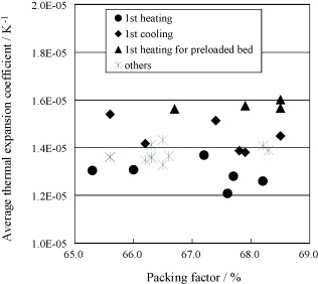
\includegraphics[width=0.65\textwidth]{images/li2tio3-thermal-expansion} 
	\caption{Effective thermal expansion of \lit~pebble beds is approximately 78\% that of the solid material.}
	\label{fig:li2tio3-thermal-expansion}
\end{figure}

However, the accuracy of the model predictions often degrade as soon as a pebble bed's granular material, grain radii distributions, or operating conditions vary from the experimentally studied packed beds. In addition, propensity for creep, crushing, and inter-particle sintering of ceramic materials alter the packing structure in ways not currently predictable with the effective material characterizations. Furthermore, effective conductivity models that consider interstitial gas often assume the gas is stagnant. Much current study in the ceramic breeder field has been on developing more accurate and robust models of heat transfer in packed beds and their unique associated phenomena when employed in fusion reactors.

\subsection{Thermo-mechanical Effects}
Reimann et al. have conducted an extensive experimental study of stress-strain relations of ceramic breeder pebble beds using an oedometric test apparatus \cite{Piazza2002811,Reimann:2002kl,Reimann:2003qc,Reimann:2002mi,Reimann:2001il}. The most significant macroscopic experimental phenomena witnessed in pebble beds is an irreversible plastic strain when load is removed, a non-linear elasticity, a pressure-dependent plasticity, and volumetric creep.  A particularly noticeable feature, clearly demonstrated in \Cref{fig:mti}, is the reduced amount of irreversible strain when subjected to additional loading cycles after the first unloading. This may suggest the existence of a semi-equilibrium packing state in the pebble bed which can be reached after applying a pre-load to account for the large strain in the first cycle of a pebble bed. This semi-equilibrium packing state is a feature which may be advantageous for use in a fusion reactor.

To study temperature effects in Reimann's studies, beds are freely heated to desired working temperatures before pressure load is applied. Under the same loading condition, beds behave much softer at higher temperatures. The bed stiffens as the pressure increases. An illustration of this phenomenon is presented in \Cref{fig:UCT} for a lithium orthosilicate pebble bed between \SIrange{50}{850}{\celsius}. At higher temperatures (such as > \SI{650}{\celsius}), a creep-like behavior becomes apparent. Creep behavior allows the pebble bed to relax and sustain higher stresses, however at eleveated temperatures we must keep in mind issues of surface sintering of pebbles. The data was used to correlate creep rate as a function of temperature, stress, and time for both lithium orthosilicate, lithium metatitanate, and beryllium pebble beds \cite{Buhler:2002qf,Reimann:2001il,Reimann2005}.


\begin{figure}[h]
    \centering
    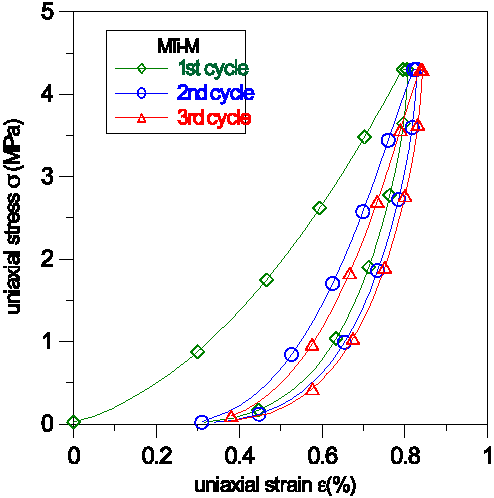
\includegraphics[width=0.65\textwidth]{images/Fig-1}
    \caption{Example of uniaxial compression testing results for lithium metatitanate pebble bed \cite{vanderlaan2011}.}
    \label{fig:mti}
\end{figure}

\begin{figure}[h]
    \centering
    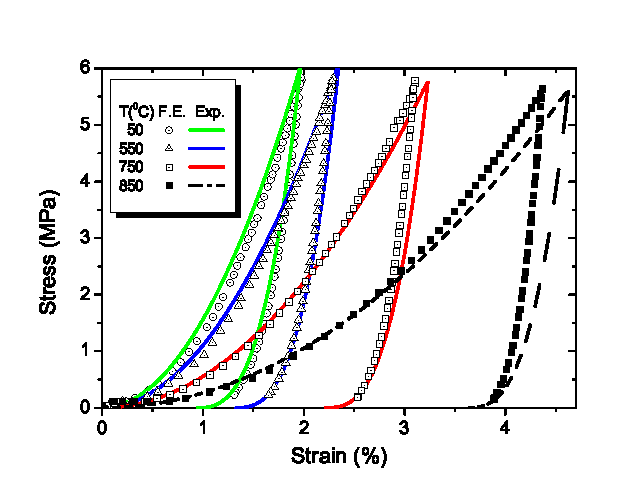
\includegraphics[width=0.65\textwidth]{images/Fig-2}
    \caption{Example of uniaxial compression testing results compared with predictions from material constitutive equations for lithium orthosilicate pebble beds at different temperatures \cite{Gan:2008kx}.}
    \label{fig:UCT}
\end{figure}


\subsubsection{Post-irradiation experiments at Petten}
The pebble bed assemblies (PBA) experiment is designed to study the effect of neutron irradiation on the thermomechanical behavior of a ceramic breeder pebble-bed under DEMO representative thermomechanical loads \cite{Magielsen2007}. This was accomplished \textit{via} analysis of changes of the in-pile temperature profiles during irradiation as wall as from the post irradiation examination of the pebble bed in the Hot Cells. Within the assemblies, there are four test elements; each resembling a small-scale mock-up of a HCPB TBM with a ceramic breeder pebble bed sandwiched between two beryllium pebble beds. Before irradiation, the beds are pre-compacted with a compressive load of \SI{3}{\mega\pascal} to ensure good settling and contact.

FEM analysis was performed to study pre-compaction procedures.  During progressive irradiation, temperatures are recorded at several locations in the ceramic breeder bed as well as other critical positions. Reviewing the recorded temperature data, when comparing the temperature in the center of the ceramic breeder pebble bed during later cycles and earlier cycles there appears to be a decrease in temperature for the exact same environmental conditions. Changes in the pebble beds and their characteristics are examined both in-pile by neutron radiography and out-of-pile by e.g. SEM during post-irradiation examination (PIE). The estimated bed height reduction from neutron radiographies over the course of the irradiation has shown 3\% of creep compaction. 

A pebble bed experiencing creep compaction is both becoming more dense as well seeing more-developed inter-pebble conduction paths. The effective thermal conductivity for a creep-compacted ceramic pebble bed is thus expected to be higher than a standard ceramic pebble bed. This phenomenon results in lower temperature gradients and a lower overall temperature magnitude, which is precisely what was observed in the experiment over the course of the cycling. 

During PIE, various microscopy preparation techniques are used to study the deformation state of the pebble beds (signs of creep compaction and sintering), formation of gas gaps between the pebble beds and structural materials, and the interaction layers between eurofer-ceramic and eurofer-beryllium. 

Figure~\ref{fig:pba} shows the cross-section of \lit~pebbles (left) and \lis~pebbles (right) post irradiation. Evident in the images is sintering of the lithium titanite and significant fracturing of the lithium orthosilicate pebbles. Importantly, however, it must be noted that the pebble beds performed reliably in spite of the changes displayed in these images.\cite{Magielsen2007} 


\begin{figure}[h]
\centering
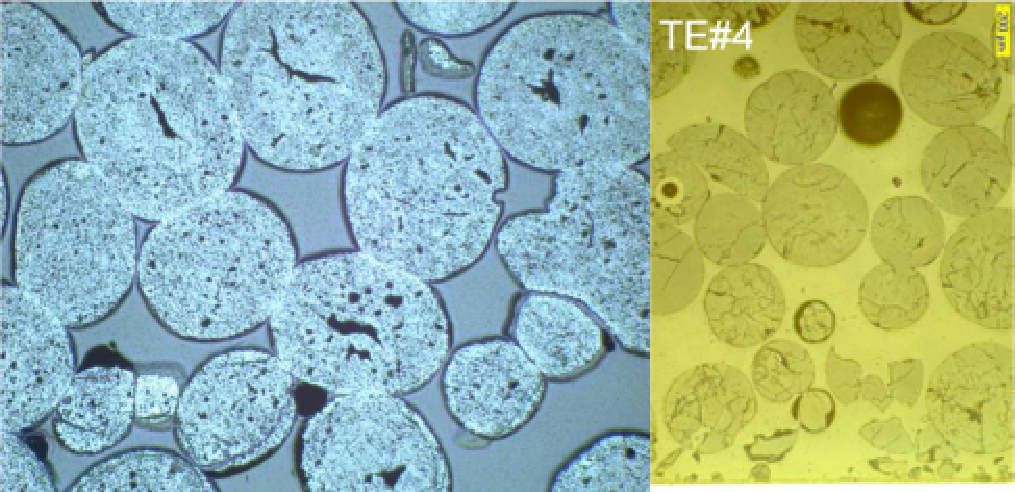
\includegraphics[width=0.65\textwidth]{images/Fig-10}
\caption{Notable features of irradiated Li$_2$TiO$_3$ and Li$_4$SiO$_4$ pebble beds from PBAcite{magielsen2011}. (Left) Demonstration of significant sintering of Li$_2$TiO$_3$ pebbles with no fracturing; the visible cracks originated from production and handling. (Right) Demonstration of cracking of Li$_4$SiO$_4$ pebbles.}
\label{fig:pba}
\end{figure}




\FloatBarrier
\section{Modeling of Solid Breeder Volumes}

In the following sections, the basis of modeling efforts for ceramic pebble beds will be introduced.

\subsection{Continuum Modeling of Packed Beds}
When we consider beds of granular material from the standpoint of engineering continuum mechanics, packed beds cannot be adequately described by traditional models of either solids or liquids alone. Under compression, a packed bed responds like a solid with non-linear elasticity and a plasticity that is history-dependent. At the same time, the packed bed can obviously not support any tensile pressure and will often behave as an extremely viscous liquid as it may fill in voids under just the force of gravity. Nevertheless, phenomenological models, derived from the volumes of collected data (such as the data described in the above sections), have been developed, using effective material properties for the ceramic pebble bed, that describe the pebble beds in an Eulerian manner that provide reliable information on the initial states of breeder volumes in the fusion reactor environment and allow reasonable design predictions of the thermomechanics of the breeding blanket. 

In spite of the shortcomings of a continuum approach, it is the only option which currently allows treatment of the pebble beds with standard finite element modeling (FEM) that can be scaled up to the breeder system. To employ FEM, mathematical models written in terms of average quantities and containing effective parameters are used. These models deduce a set of constitutive equations to be implemented in the framework of a finite element code.  There are two major variants of phenomenological modeling approaches developed among institutions, including: (1) A non-linear elastic model and a modified Drucker-Prager-Cap theory for plastic strain \cite{Gan2007189,Fokkens2003}; and (2) A hyper-porous non-linear elastic model and a Gurson model for the plastic model \cite{DellOrco:2007hc,DellOrco:2010zr,DiMaio20081287}. Another approach was taken by Ref.\cite{Fokkens2003} wherein the authors employed two different elasticity laws for the loading and unloading branches. Alongside the development of the modeling techniques, several large scale pebble bed thermomechanics experiments were conducted. These experiments were intended to reveal the underlined thermomechanical characteristics of ceramic breeder pebble beds, and provide data for benchmarking the developed models. The vast amount of work done on modeling the pebble beds in the FEM framework can be found in literature. \cite{DellOrco:2007hc,DellOrco:2010zr,DiMaio20101234,Gan:2009vn,Gan:2010lh,Gan:2010kc,Gan2007189} 



\section{Discrete Modeling of Packed Beds}
Aided by the acceleration and availability of computational power, many researchers of granular heat transfer have shifted their attention to studies of the interacting physics on pebble-scales with the discrete element method (DEM). In this approach, we interrogate heat transfer on the scale of contact conductance between interacting particles and directly model transient behaviors of packed beds. This approach has the advantage providing the capability to monitor transient changes to meta-stable packing structures of pebble beds; changes such as plastic rearrangement, inter-particle sintering/creep, fragmentation of pebbles, \textit{etc.}.

DEM models have also been shown to efficiently couple to either volume-averaged fluid models or models of the entire tortuous fluid flow through the porous network of packed beds. Refs\cite{Annabattula2011,Lu2000b,An20072233,gan20072233,VanLew2014,VanLew2015} contain recent examples of application DEM models for solid breeder research.



\subsection{Particle Dynamics}\label{sec:particle-dynamics}

The grains in our system are allowed translational and rotational degrees of freedom. In a packed bed, we can restrict our attention to local forces between particles; neglecting, say, non-contact forces such as, van der Waals, electrostatic, or for the time being any fluid interaction forces. Assuming we know the contact forces acting upon particle $i$, Newton's equations of motion are sufficient to describe the particle kinematics. For translation and rotational degrees of freedom, the equations are:,
\begin{subequations}\label{eq:newtons-second}
\begin{align}
	m_i  \ddt{\vec{r}_i}   & = m_i\vec{g} + \vec{f}_i \label{eq:newton-translational} \\
	I_i\dt{\vec{\omega}_i} & = \vec{T}_i \label{eq:newton-rotational}
\end{align}
\end{subequations}
where $m_i$ is the particle mass, $\vec{r}_i$ its location in space, $\vec{g}$ is gravity, $I_i$ is the particle's moment of inertia, and $\vec{\omega}_i$ its angular velocity.

The net contact force, $\vec{f}_i$, represents the sum of the normal and tangential forces from the total number of contacts, $Z$, acting on this grain.
\begin{equation}
 	\vec{f}_i = \sum_{j=1}^{Z} \vec{f}_{n,ij} + \vec{f}_{t,ij}
 \end{equation} 
and the net torque, $\vec{T}_i$, is similarly,
\begin{equation}
	\vec{T}_i = -\frac{1}{2}\sum_{j=1}^{Z} \vec{r}_{ij} \times \vec{f}_{t,ij}
\end{equation}

When Cundall \& Strack first proposed the discrete element method, they used a linear spring-dashpot structure which saw normal and tangential forces written as,
\begin{subequations}
\label{eq:dem-forces}
\begin{align}
	\vec{f}_{n,ij} &= k_{n,ij} \delta_{n,ij}\vec{n}_{ij} - \gamma_{n,ij} \vec{u}_{n,ij} 	\label{eq:normal-force} \\
	\vec{f}_{t,ij} &= k_{t,ij} \delta_{t,ij}\vec{t}_{ij} - \gamma_{t,ij} \vec{u}_{t,ij} 	\label{eq:tangential-force}
\end{align}
\end{subequations}
where Cundall \& Strack defined the stiffness coefficients $k$ as constants and local damping coefficients $\gamma$ were proportional to them, $\gamma \propto k$, to allow dissipation of energy and the system to reach an equilibrium. 

Relative normal and tangential velocities, respectively, are decomposed from particle velocities,
\begin{subequations}
\label{eq:dem-velocities}
\begin{align}
	\vec{u}_{n,ij} &= (-(\vec{u}_i-\vec{u}_j)\cdot\vec{n}_{ij})\vec{n}_{ij} \\
	\vec{u}_{t,ij} &= (-(\vec{u}_i-\vec{u}_j)\cdot\vec{t}_{ij})\vec{t}_{ij}
\end{align}
\end{subequations}
with the unit vector $\vec{n}_{ij}$ pointing from particle $j$ to $i$

Surfaces of the two particles are allowed to virtually pass through each other (no deformation) resulting in normal and tangential overlaps of,
\begin{subequations}
\label{eq:dem-overlaps}
\begin{align}
	\delta_{n,ij} &= (R_i + R_j) - (\vec{r}_i -\vec{r}_j)\cdot \vec{n}_{ij} \\
	\delta_{t,ij} &= \int_{t_{c,0}}^{t} \vec{u}_{t,ij}\,\mathrm{d}\tau 
\end{align}
\end{subequations}
where the fictive tangential overlap, $\delta_{t,ij}$, is truncated to so the tangential and normal forces obey Coulomb's Law, $\vec{f}_{t,ij} \le \mu_i \vec{f}_{n,ij}$ with $\mu$ as the coefficient of friction of the particle.

Thus the approach of DEM is relatively simple: calculate interaction forces between particles with \Cref{eq:dem-forces} based on the kinematics of velocity and position of interacting particles from \Cref{eq:dem-velocities} and \Cref{eq:dem-overlaps}, respectively, then update the positions based on the forces. As DEM evolved and drew attention of more researchers, more complex formulas governing the spring-dashpot coefficients of \Cref{eq:dem-forces} emerged. But the core approach remained the same and the models all fall into the same family of so-called `soft particle' models of DEM. A well-composed summary of the different DEM force models is given by Zhu et al..\cite{Zhu2007}

The method used in this work fits into the computational skeleton of Cundall and Strack's method but with non-linear spring-dashpot coefficients defined by simplified Hertz-Mindlin-Deresiewicz model. In this model, the normal-direction stiffness coefficient of \Cref{eq:normal-force} is based on the Hertzian contact law. The tangential-direction stiffness coefficient follows from Brilliantov \cite{Brilliantov1996, Zhu2007, Langston1995}. Together, the spring coefficients are,
\begin{subequations}
\begin{align}
	k_{n,ij} &= \frac{4}{3}E_{ij}^*\sqrt{R_{ij}^*\delta_{n,ij}} \\
	k_{t,ij} &= 8 G_{ij}^*\sqrt{R_{ij}^*\delta_{t,ij}}
\end{align}
\end{subequations}
where $E_{ij}^*$ is the pair Young's modulus, $G_{ij}^*$ is the pair bulk modulus, and $R_{ij}^*$ is the relative radius. The terms are defined as,
\begin{subequations}
\begin{align}
	\frac{1}{E^*} &= \frac{1-\nu_1^2}{E_1} + \frac{1-\nu_2^2}{E_2} \\
	\frac{1}{R^*} &= \frac{1}{R_1} + \frac{1}{R_2} \\
	\frac{1}{G^*_{ij}} &= \frac{2(2+\nu_i)}{E_i} + \frac{2(2+\nu_j)}{E_j}
\end{align}
\end{subequations}

Similar to Cundall \& Strack's formulation, damping coefficients, $\gamma$, are included to account for energy dissipated from the collision of two particles \cite{DiRenzo2004, Tsuji1992, Tsuji1993}. Whether the damping coefficient is local or global and the exact form of the coefficient is more important for loosely confined granular systems and dictates the way the system approaches an equilibrium state \cite{Makse2004}. For the case of our tightly packed pebble beds, it suffices to use the efficient form of Refs.\cite{Dippel1996, Makse2004, Brilliantov1996, Zhang2005, Zhu2007},
\begin{subequations}
\begin{align}
	\gamma_n &= \sqrt{5}\beta_\text{diss}\sqrt{m^*k_{n,ij}} \\
	\gamma_t &= \sqrt{\frac{10}{3}}\beta_\text{damp}\sqrt{k_{t,ij} m^*}
\end{align}
\end{subequations}
with $\beta_\text{damp}$ as the damping ratio, and the pair mass, $\frac{1}{m^*} = \frac{1}{m_i} + \frac{1}{m_j}$. For a stable system with $\beta_\text{damp} < 1$, the damping ratio is related to the coefficient of restitution, $e$, as
\begin{equation}
	\beta_\text{diss} = -\frac{\ln{e}}{\sqrt{\ln^2{e}+\pi^2}}
\end{equation}

Systems to be solved by DEM models are therefore well-defined after specifying the few material properties of $E$, $\nu$, $\rho$, and $R_p$ and the interaction properties of $\mu$ and $e$.

Having expressed the contact mechanics of the discrete element method, we now must integrate the kinematic equations of the particles to resolve their evolutions. The most common means of marching in time with DEM is the velocity-Verlet algorithm \cite{Kruggel-Emden2008}. In this algorithm, \Cref{eq:newtons-second} are integrated with half-steps in velocity, full steps in position, and then finally the full step in velocity. In practice, the two half-steps in velocity are often compressed into a single, full step.


%~~~~~~~~~~~~~~~~~~~~~~~~~~~~~~~~~~~~~~~~~~~~~~~~~~~~~~~~~~~~~~~~~~~~~~~~~~~~~~~~~~~~~~~~~~~~~~~~~~~~~~~~~~~
% new subsection
%~~~~~~~~~~~~~~~~~~~~~~~~~~~~~~~~~~~~~~~~~~~~~~~~~~~~~~~~~~~~~~~~~~~~~~~~~~~~~~~~~~~~~~~~~~~~~~~~~~~~~~~~~~~
\subsection{Granular Heat Transfer in DEM}\label{sec:dem-heat-transfer}

In a way analogous to handling particle momentums with Newton's laws of motion, Lagrangian tracking of particle energy is obtained \textit{via} the first law of thermodynamics. Each particle is treated as a single distinct object and thus internal temperature gradients are assumed negligible. The temperature of particle $i$ is governed by
\begin{equation}\label{eq:thermoFirstLaw}
	m_iC_i\frac{\mathrm{d}T_i}{\mathrm{d}t} = Q_{s,i} + Q_{i}
\end{equation}
where $m$ and $C$ are the mass and the specific heat of the solid, respectively. Heat generation inside the particle is input with $Q_{s}$ and the total heat transferred to/from particle $i$ \textit{via} conduction to all, $Z$, neighboring particles, is
\begin{equation}
	Q_i = \sum_{j=1}^Z Q_{ij}
\end{equation}

Assuming the particles are spherical, smooth, elastic, in vacuum, and we neglect radiation transfer between them, for two particles at temperatures $T_i$ and $T_j$, we quantify the amount of energy transferred between them with a contact conductance, $H_c$:
\begin{equation}\label{eq:pebble-conduction-heat-transfer}
    Q_{ij} = H_{c}(T_i - T_j)
\end{equation}
where $H_c$ is a contact conductance term defining the squeezing of heat transfer through contact areas,\cite{Batchelor1977,Cheng19994199}
\begin{equation}\label{eq:cheng-modification-batchelor}
    H_c = 4k^*a = 4k^* \left(\frac{3}{4}\frac{R^*}{E^*}\right)^{1/3}F_n^{1/3}
\end{equation}
where $\frac{1}{k^*} = \frac{1}{k_i} + \frac{1}{k_j}$ and $k_{i/j}$ are conductivities of contacting solids and $a$ is the radius of contact. Because we have assumed smooth, elastic, spherical solids, with Hertz theory, contact radius can be found as a function of contact normal force, $F_n$,
\begin{equation}
    a =  \left(\frac{3}{4}\frac{R^*}{E^*}\right)^{1/3}F_n^{1/3} 
\end{equation}
where, as before, $\frac{1}{E^*} = \frac{1-\nu_1^2}{E_1} + \frac{1-\nu_2^2}{E_2}$ and $\frac{1}{R^*} = \frac{1}{R_1} + \frac{1}{R_2}$. 

The total heat transferred out of a single particle with $Z$ contacts, due to contact conductance, is then simply the summed contribution of individual contacts, 
\begin{equation}
    Q_i = \sum_j^Z Q_{ij}
\end{equation}

\subsection{DEM Examples}
In a recent study, we considered the changes to heat transfer as packing structures evolve due to fragmentation of individual pebbles.



\begin{figure}[h]
        \centering
        \begin{subfigure}[t]{0.45\textwidth}
                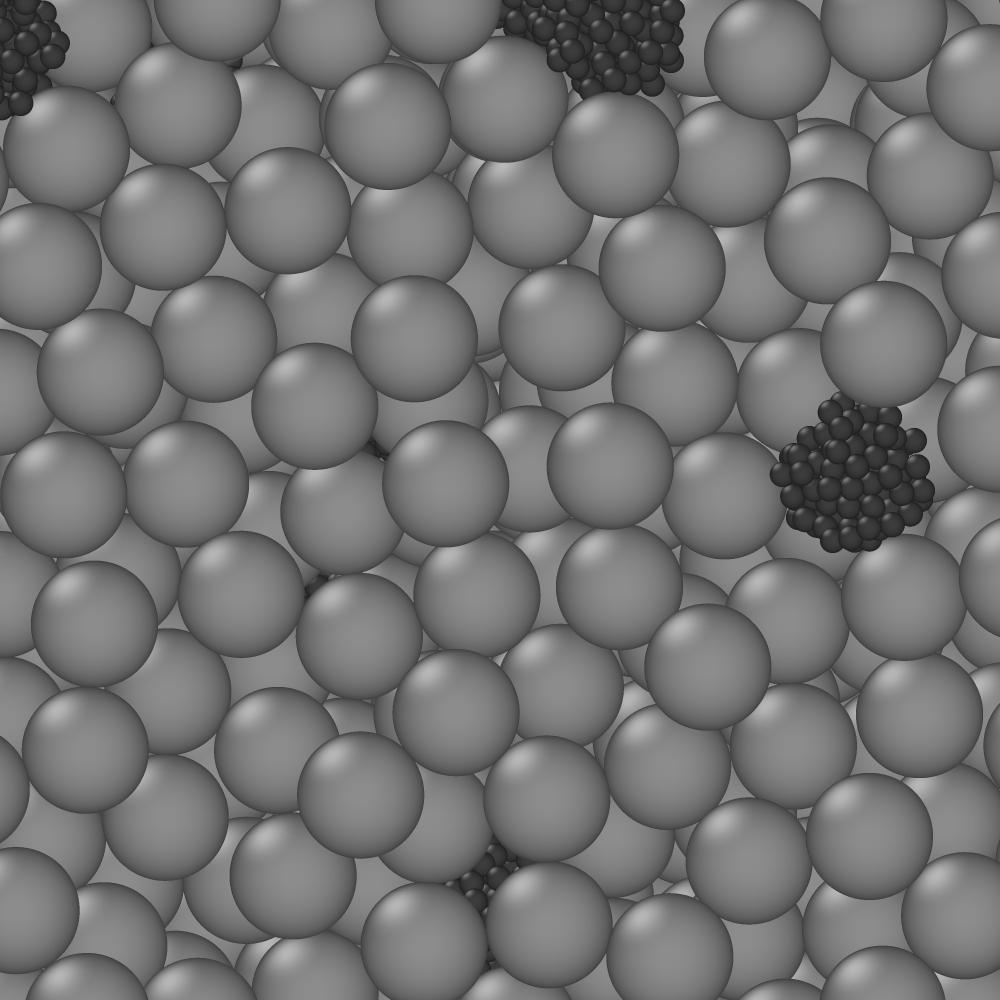
\includegraphics[width=\textwidth]{images/crushed_initial}
                \caption{Initial placement of fragments.}
                \label{fig:crushed-initial}
        \end{subfigure}%
        ~
        \begin{subfigure}[t]{0.45\textwidth}
                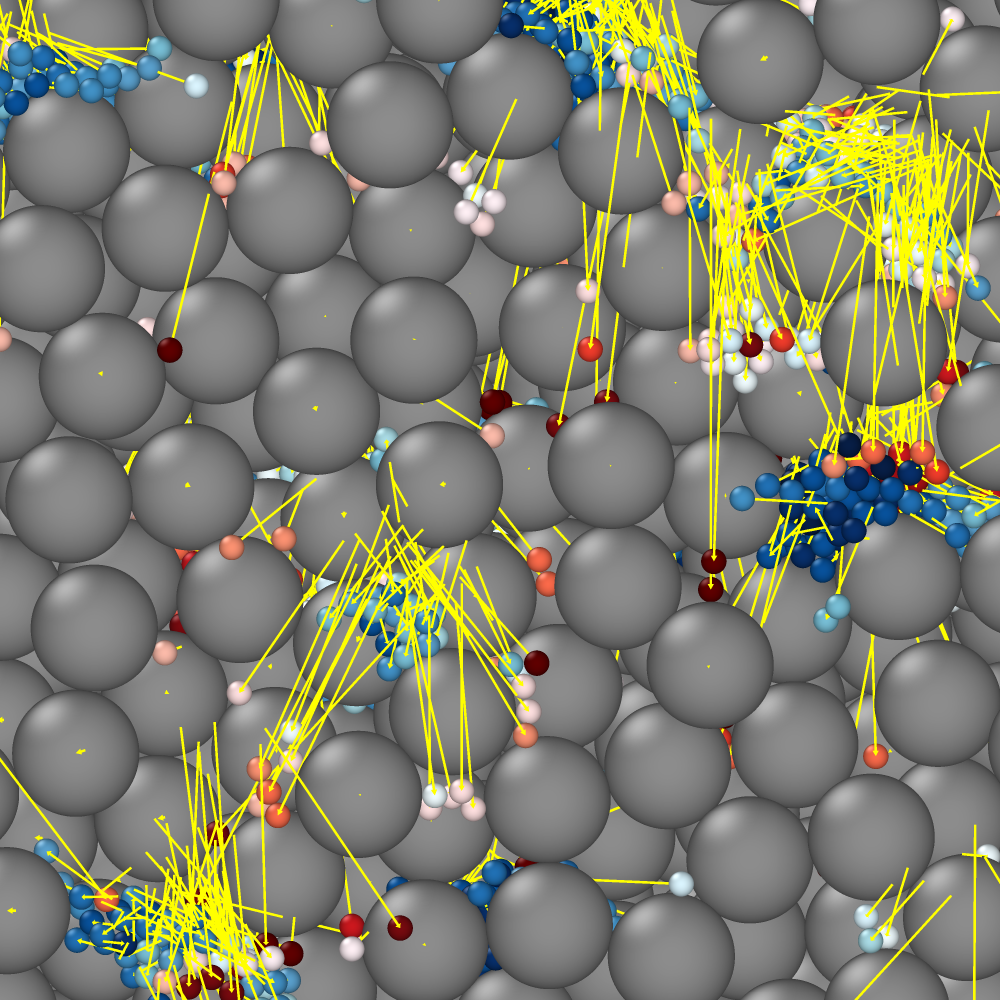
\includegraphics[width=\textwidth]{images/crushed_final}
                \caption{Settling of fragments.}
                \label{fig:crushed-final}
        \end{subfigure}
        \caption{Vector displacements of fragments after resettling.}\label{fig:crushed-travel}
\end{figure}

\begin{figure}[!t]
    \centering
    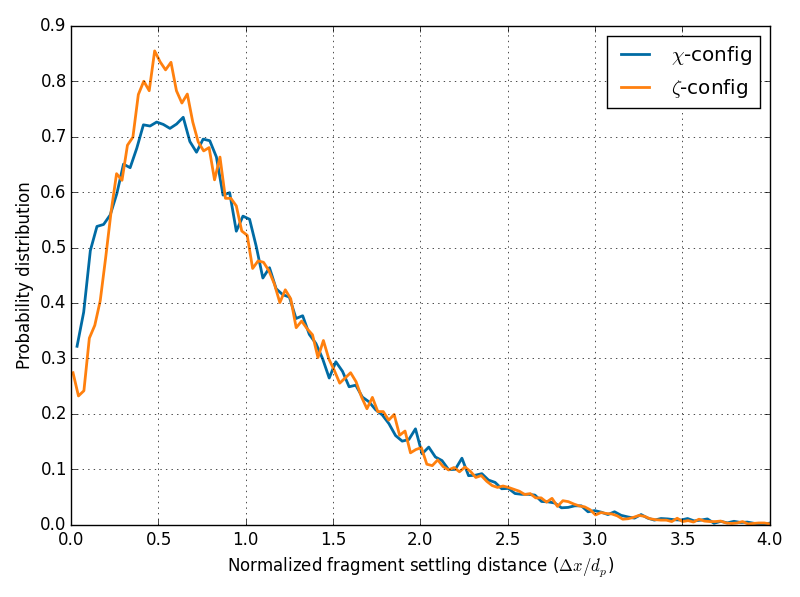
\includegraphics[width = 0.65\textwidth]{images/displacement_histograms.png}
    \caption{Normalized displacement histograms. $\chi$-config: 59.7\% of fragments travel up to \SI{1}{\milli\meter} and 8.2\% travel more than \SI{2}{\milli\meter}; $\zeta$-config: 60.7\% of fragments travel up to \SI{1}{\milli\meter}, 7.9\% travel more than \SI{2}{\milli\meter}.}\label{fig:displacement_hists}
\end{figure}


% deltas~~~~~~~~~~~~~~~~~~~~~~~~~~
\begin{figure}[!t]
    \centering
    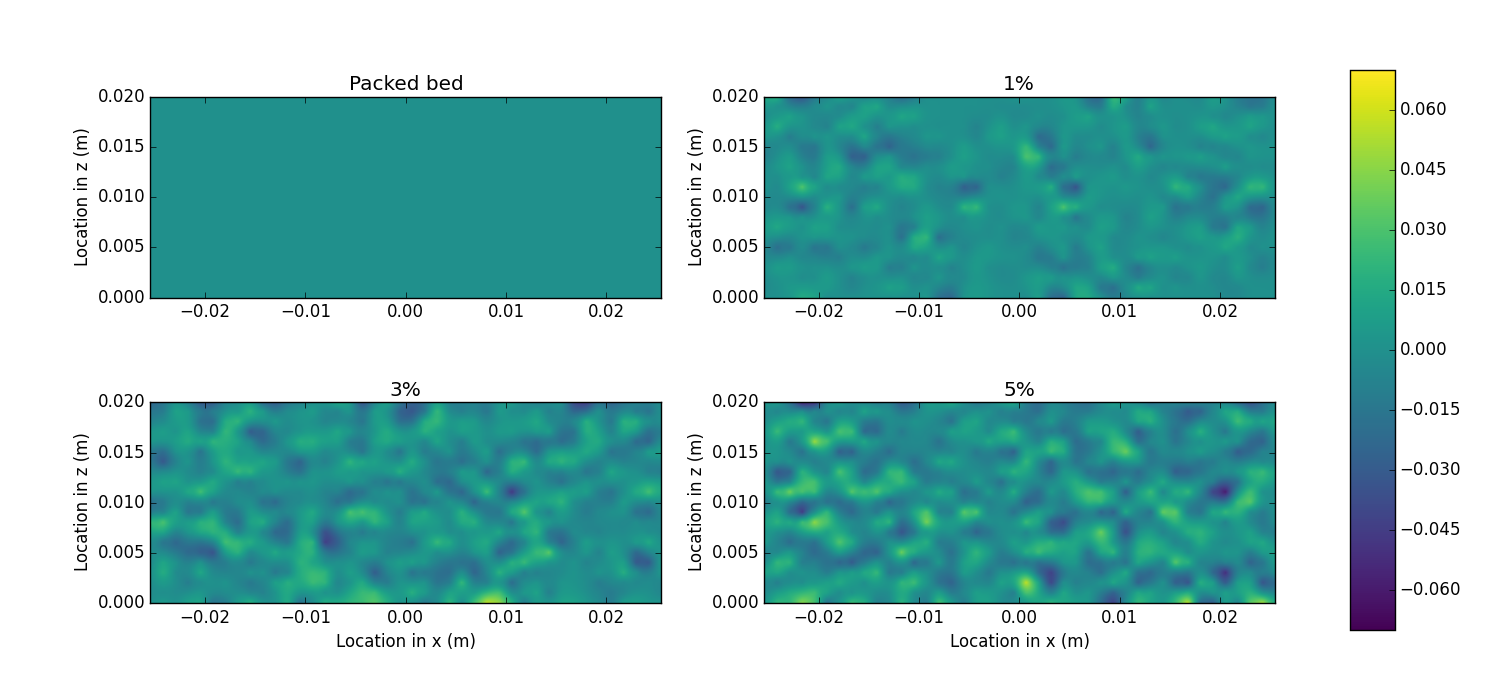
\includegraphics[width = \textwidth]{images/z-62-r23-1-deltas.png}
    \caption{Distribution of local changes in packing fraction ($\phi_{\eta} - \phi_i$) for $\zeta$-config, $\phi = 0.62$, $r^* = 0.32$}\label{fig:z-62-r23-deltas}
\end{figure}

\begin{figure}[!t]
    \centering
    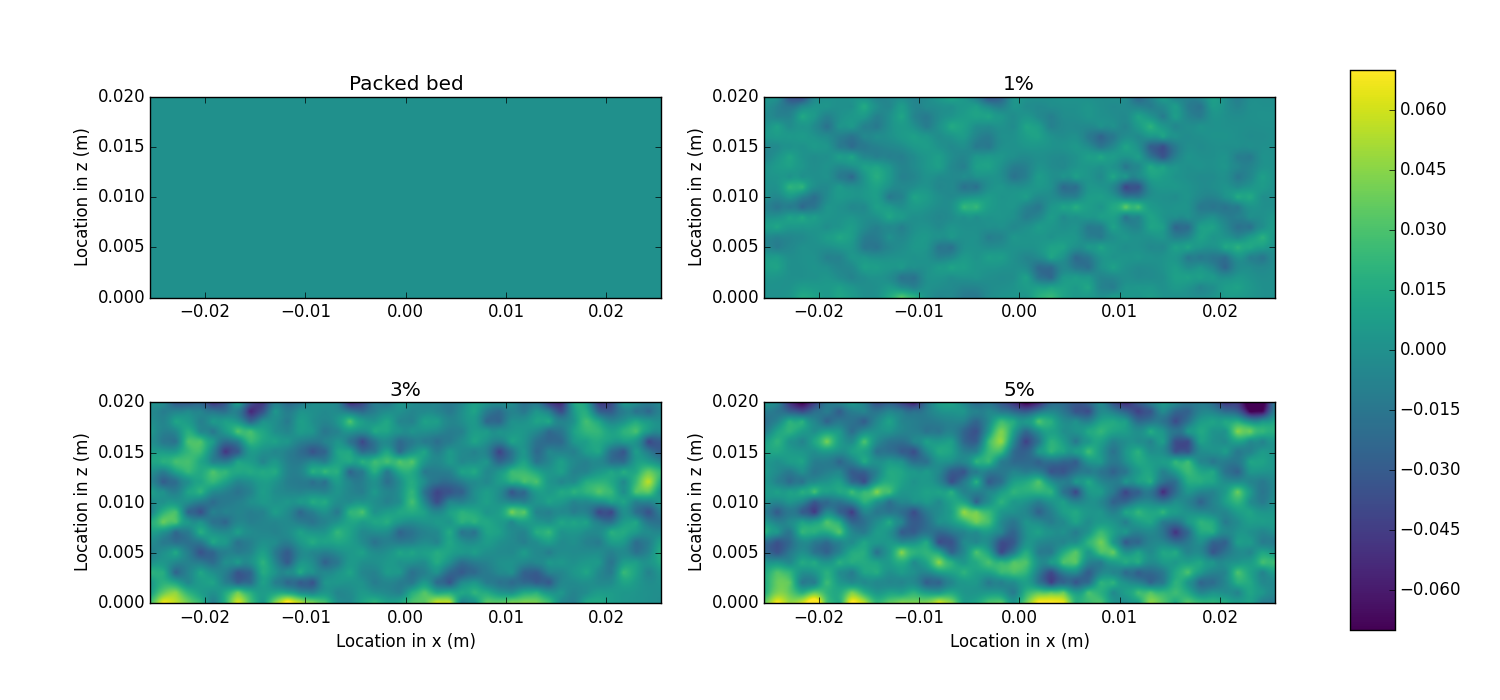
\includegraphics[width = \textwidth]{images/z-62-r125-1-deltas.png}
    \caption{Distribution of local changes in packing fraction ($\phi_{\eta} - \phi_i$) for $\zeta$-config, $\phi = 0.62$, $r^* = 0.2$}\label{fig:z-62-r125-deltas}
\end{figure}

\begin{figure}[!t]
    \centering
    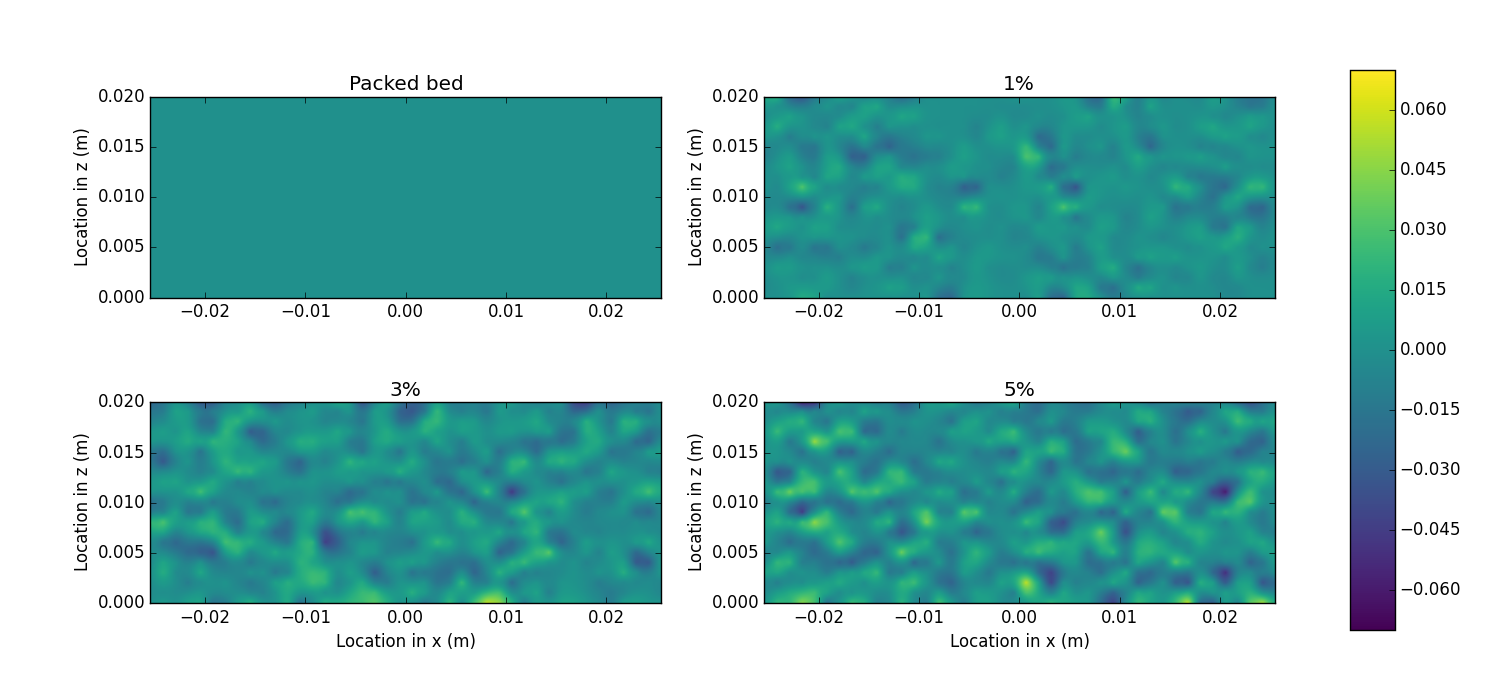
\includegraphics[width = \textwidth]{images/z-62-r23-1-deltas.png}
    \caption{Distribution of local changes in packing fraction ($\phi_{\eta} - \phi_i$) for $\zeta$-config, $\phi = 0.64$, $r^* = 0.32$}\label{fig:z-624-r23-deltas}
\end{figure}

\begin{figure}[!t]
    \centering
    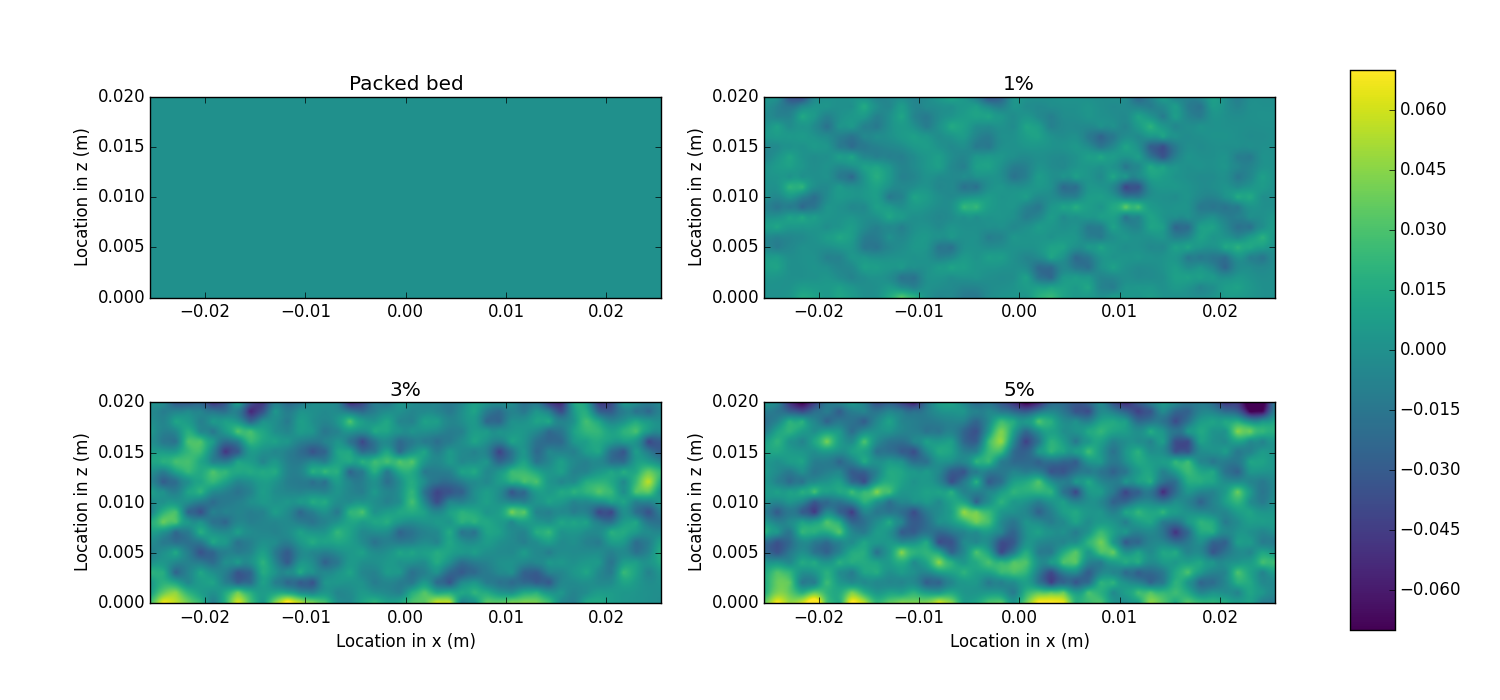
\includegraphics[width = \textwidth]{images/z-62-r125-1-deltas.png}
    \caption{Distribution of local changes in packing fraction ($\phi_{\eta} - \phi_i$) for $\zeta$-config, $\phi = 0.64$, $r^* = 0.2$}\label{fig:z-624-r125-deltas}
\end{figure}
% deltas~~~~~~~~~~~~~~~~~~~~~~~~~~


\bibliography{library.bib}
\bibliographystyle{plain}

\end{document}